\documentclass[
	11pt, % Default font size, select one of 10pt, 11pt or 12pt
	fleqn, % Left align equations
	b5paper,
	% Paper size, use either 'a4paper' for A4 size or 'letterpaper' for US letter size
	%oneside, % Uncomment for oneside mode, this doesn't start new chapters and parts on odd pages (adding an empty page if required), this mode is more suitable if the book is to be read on a screen instead of printed
]{LegrandOrangeBook}

% Book information for PDF metadata, remove/comment this block if not required 
\hypersetup{
	pdftitle={Title}, % Title field
	pdfauthor={Author}, % Author field
	pdfsubject={Subject}, % Subject field
	pdfkeywords={Keyword1, Keyword2, ...}, % Keywords
	pdfcreator={LaTeX}, % Content creator field
}

\DeclareUnicodeCharacter{0301}{*************************************}

% Bibliography files
\addbibresource{Aging_Schelling.bib}
\addbibresource{Aging_Threshold.bib}
\addbibresource{Aging_STM.bib}

\definecolor{ocre}{RGB}{0, 153, 0} % Define the color used for highlighting throughout the book

\chapterimage{} % Chapter heading image
\chapterspaceabove{6.5cm} % Default whitespace from the top of the page to the chapter title on chapter pages
\chapterspacebelow{6.75cm} % Default amount of vertical whitespace from the top margin to the start of the text on chapter pages

%----------------------------------------------------------------------------------------

\begin{document}

%----------------------------------------------------------------------------------------
%	COVER PAGE
%----------------------------------------------------------------------------------------

\begin{titlepage}
    %\pdfbookmark[1]{\myTitle}{titlepage}
    % if you want the titlepage to be centered, uncomment and fine-tune the line below (KOMA classes environment)
    	\large

        \begin{center}
            \sffamily
            \includegraphics[width=.35\textwidth]{Figs/uib.png}
        
            \vspace*{.05\textheight}

			{\Huge\bfseries DOCTORAL THESIS} \\
			{\Large \bfseries 2024}

            \vspace*{.15\textheight}

			\begingroup
				{\Huge\bfseries Aging in the idealista model for complex systems housing \par}
			\endgroup

            \vfill

            {\Large \bfseries David Abella Bujalance}
        \end{center}
\end{titlepage}

%----------------------------------------------------------------------------------------
%	TITLE PAGE
%----------------------------------------------------------------------------------------

\thispagestyle{empty}

\begin{titlepage}
    %\pdfbookmark[1]{\myTitle}{titlepage}
    % if you want the titlepage to be centered, uncomment and fine-tune the line below (KOMA classes environment)
    \large

    \hfill
    \begin{minipage}[c][0.2\textheight]{0.45\textwidth}
        \includegraphics[width=.75\textwidth]{Figs/uib.png}
	\end{minipage}
    \hfill
    \begin{minipage}[c][0.2\textheight]{0.45\textwidth}
        \includegraphics[width=1\textwidth]{Figs/ifisc.pdf}
    \end{minipage}
    \hfill
	{\centering\sffamily
    \vspace*{.1\textheight}
        
    {\Huge\bfseries DOCTORAL THESIS} \\
    {\Huge\bfseries 2024}
        
    \bigskip

    {\Large\bfseries Doctoral programme in Physics} \\

    \vfill
        
    \begingroup
        {\Huge\bfseries Aging in the idealista model for complex systems housing \par}
    \endgroup

    \bigskip
            
    {\Large\bfseries David Abella Bujalance}
            
    \vfill
	}

    \begin{flushleft}
		\sffamily
        \textbf{Thesis Supervisor:} Jos\'e Javier Ramasco Sukia \\
        \textbf{Thesis Supervisor:} Maxi San Miguel \\
        \textbf{Thesis Tutor:} Crist\'obal L\'opez S\'anchez\\

        \vfill

        Doctor by the Universitat de les Illes Balears \\
    \end{flushleft}
\end{titlepage}

%----------------------------------------------------------------------------------------
%	COPYRIGHT PAGE
%----------------------------------------------------------------------------------------

\thispagestyle{empty} % Suppress headers and footers on this page

~\vfill % Push the text down to the bottom of the page
\sffamily

\noindent \textbf{Supervisors:}

\noindent Jos\'e Javier Ramasco Sukia

\noindent Maxi San Miguel \\

\noindent David Abella Bujalance.

\noindent \textit{Aging in the idealista model for complex systems housing.} \copyright

\noindent Palma de Mallorca, June 2024
\pagebreak

%----------------------------------------------------------------------------------------
%	DEDICATION
%----------------------------------------------------------------------------------------
\thispagestyle{empty}

\vspace*{8 cm}

\begin{flushright}
    \sffamily\Large
    \textit{
    A les meves germanes, Adriana i Ivet,\\
    per ser-hi sempre, per estimar-me, per fer-me riure, \\
    i per totes les vegades que heu intentat esbrinar que es un sistema complex.\\
    }
\end{flushright}
\newpage
\thispagestyle{plain} % empty
\mbox{}

%----------------------------------------------------------------------------------------
%	INTERNATIONAL PhD PROGRAM IN PHYSICS
%----------------------------------------------------------------------------------------

\newpage
\thispagestyle{plain} % empty
\mbox{}
\thispagestyle{empty}

Dr Jos\'e Javier Ramasco of the Consejo Superior de Investigaciones Cient\'ificas (CSIC) and Dr Maxi San Miguel of the Universitat de les Illes Balears (UIB)

\vspace*{2 cm}

WE DECLARE:

\vspace*{1 cm}

That the thesis titles \textit{Aging in the idealista model for complex systems housing}, presented by David Abella Bujalance to obtain a doctoral degree, has been completed under my supervision and meets the requirements to opt for an International Doctorate.

\vspace*{2 cm}

For all intents and purposes, I hereby sign this document.

\vspace*{2 cm}

Signature

\vspace*{3 cm}

      Dr. Jos\'e Javier Ramasco Sukia              \hfill Dr. Maxi San Miguel


\vspace*{0.1 cm}

        Thesis Supervisor              \hfill Thesis Supervisor

\vspace*{1 cm}

        Palma de Mallorca, June 2024

\vfill
\newpage
\thispagestyle{plain} % empty
\mbox{}

%----------------------------------------------------------------------------------------
%	ACKNOWLEDGEMENTS
%----------------------------------------------------------------------------------------

\pagebreak
\frontmatter
\thispagestyle{empty}
\phantomsection
\addcontentsline{toc}{chapter}{Acknowledgements}
\textbf{ \huge Acknowledgements}

\vspace*{0.5 cm}

I want to express my sincere and profound gratitude to my supervisors, Maxi San Miguel and José J. Ramasco. Their guidance and academic support have been fundamental during this thesis and have given me a different perspective on both work and life. Maxi, with his experience and his questions on key details, has provided invaluable insight, while José has been a constant and understanding guide. I appreciate that his door is always open for discussions that can go off on tangents and end up who knows where. I also want to deeply thank them for the financial support they have provided. Not having been lucky with doctoral scholarships, I have been able to complete this thesis thanks to their projects without having to worry about money. Their generosity has been key to completing this thesis. A special thanks to Vincenzo Nicosia, with whom I had the opportunity to do a research stay in London. Collaborating with him truly gave me good motivation and allowed me to start very interesting projects and be part of idea development. I am very excited to see where our work from those months will lead. Regarding the scientific aspect, I also want to thank other scientists with whom I have had very inspiring conversations along this journey, such as Juan Fernández Gracia, Raúl Toral, Konstantín Klemm, and Sandro Meloni. Conversations with them have been a constant source of inspiration and learning for me.

My first steps on this path began with the master's in Complex Systems. There, I had the fortune of enjoying the company of great students like Alex, Robert and Marius, Miguel, and those from the Pisito at that time: Javi, Medi, Jorge, and Ana. During that time, I am grateful for the good atmosphere we had among all of us, which motivated me to stay in this field. Alex has not only been a friend from the master's but we have made this entire journey together, helping each other, sharing dramas and laughs, with "chill" routes both to Massanella and Sabotage, and being victims of FPI-CAIB injustices year after year. I also want to mention Miguel with special affection, one of the most random people I know, and I really appreciate the random videos at mid-morning and Google Maps curiosities.

During the doctorate, I have been fortunate to have extraordinary companions like Manu. We have shared many conversations (when I say many, I mean many), both at the scientific and personal levels, supporting each other at all times and chatting about our rare epidemics. The beers at Sepia and the "cine" are moments I cherish dearly. I also want to thank Mar, a person with a very clear view of the world that inspires me and has made me laugh a lot over this time. Having a shoulder like hers to cry on is very comforting. I also want to thank Gorka for making me laugh, keeping me up to date with www.internet.com. We have spent great moments together, discussing all possible methods of community detection and why none of them are good. And of course, Fer, a companion of long talks discussing a thousand topics. I don't think there's any project at IFISC that we haven't discussed and talked about how we would do it ourselves. I am very grateful you came into my life because I was a bit lost with the doctorate when you arrived. Having such an academic person like you by my side has helped me follow this path. Plus, I'm fascinated with his incredible ability to sleep in strange places. I also appreciate having had Adrià by my side, the most restless person I have ever seen, I want to thank him in particular for the last Poster Party and for both ADSL. I also want to mention Alba and Manu P. for the laughs on the boat, even though we often drifted and the boat had many damp spots, sailing the waves together was great, and I have fond memories. As friends and companions on this journey, I also want to mention Bea, Mar Ferri, Pau, Pablo, Maria, Javi, Rodri, Irene, Lisa, José (Pepe), and Carmela. We have had a great time together, and I feel very grateful to have done the doctorate with you. I also want to especially thank my group from the Summoner's rift: Jesús, Manu, and Jun. Someday we will publish a paper on this (or not), and it will be epic. And if not, no one will take away the fun we've had.



I want to express my gratitude to IFISC for having such a friendly environment among Ph.D. students, for the Poster Party, and the winter and summer solstice. I also especially thank the ``Zulo''. When I arrived, S17 was an almost empty room, and we made that room our home, our headquarters from which to create combative posters. Perhaps one of the few theoretical physics offices in the world with an extractor hood.

Of course, I thank my father, my mother, my sister Adriana, Ivet, my new nephew Aleix, who is younger than this thesis, Josepa, Pau, and Mimi. You are my family; thank you for listening to me talk about work without understanding anything I say, and thank you for all the support until reaching here, both economic and emotional.

Also, I need to mention Rosa and Pau. You are love, and you make me very happy. I like being able to vent with you, and I am glad to thank you now for the role you have played, whether calming my worries about work or contracts or simply listening to me talk about my little things.

\thispagestyle{empty}

Finally, I want to thank to Riki, you have been the cornerstone of this period. Without you, there is no thesis; without you, I don't know what I would be doing with my life. I am very grateful for the very long audios you have listened to, talking for the thousandth time about how badly my day was due to work-related frustration, for being there supporting me from a distance or in person, for understanding my needs and helping me, for being understanding with this way I function both personally and work-wise. For everything, I thank you for walking this path with me. This thesis is as much mine as it is yours.


\vfill
\newpage
\thispagestyle{plain} % empty
\mbox{}

%----------------------------------------------------------------------------------------
%	RESUM
%----------------------------------------------------------------------------------------

\pagebreak
\thispagestyle{empty}
\section*{Resum}

En els sistemes complexos distribuïts, els sistemes de memòria transaccional distribuïda (DTM) són una eina molt útil per a la programació concurrent. Aquests sistemes permeten als desenvolupadors de software escriure codi concurrent sense haver de preocupar-se per la gestió de la memòria compartida. A més, els DTM ofereixen una interfície molt senzilla per a la programació concurrent, ja que permeten als desenvolupadors de software escriure codi concurrent de forma semblant a com ho farien si el codi fos seqüencial. Tot i això, els DTM no són una eina perfecta, ja que tenen un rendiment molt inferior al de les estructures de dades distribuïdes. A més, els DTM no són capaços de gestionar estructures de dades distribuïdes de forma eficient. Per aquest motiu, els DTM no són una eina adequada per a la programació de sistemes distribuïts.

\vfill

%----------------------------------------------------------------------------------------
%	RESUMEN
%----------------------------------------------------------------------------------------

\pagebreak
\thispagestyle{empty}
\phantomsection
\addcontentsline{toc}{chapter}{Resumen}
\textbf{ \huge Resumen}

\vspace*{0.5cm}

En esta tesis doctoral, investigamos la compleja interacción entre las dinámicas temporales asociadas con la memoria y la costumbre, y sus efectos en los sistemas sociales y económicos. Para ello, combinamos modelos teóricos, para explorar las implicaciones de la costumbre en modelos de umbrales (presión social), y el análisis empírico, para abordar el impacto de los patrones temporales y espaciales en sistemas complejos reales, tomando como caso de estudio el mercado inmobiliario.

La investigación en esta tesis se estructura en dos partes principales. En la primera parte, nos centramos en hacer modelos teóricos para entender como el acostumbrarse a un estado (representativo de una opinión, comportamiento, etc.) influye otros mecanismos de cambio social y qué implicaciones tiene este mecanismo en el comportamiento emergente del sistema. Acostumbrarse en este contexto se entiende como una resistencia creciente a cambiar el estado actual, lo que también puede entenderse como un recuerdo de los estados pasados. En otras palabras, como más tiempo lleve un agente con un estado, menos probable es que cambie este. En esta tesis, analizamos la costumbre en modelos de umbrales, donde el mecanismo de cambio social es la presión social (modelada como un umbral). Estos modelos son usados para describir 3 fenómenos sociales diferentes: segregación, difusión de innovaciones y la llegada al consenso. En el modelo de segregación de Sakoda-Schelling, los efectos de acostumbrarse se entienden como una persistencia a quedarse en la residencia actual como más tiempo un agente haya estado satisfecho allí. Esta modificación es capaz de llevar el sistema de un estado mixto a uno segregado, por lo tanto, es capaz de romper la transición de fase mixta-segregada presente en el modelo original. A pesar de que la costumbre promueve la segregación, el crecimiento de dominios en la fase segregada es lento, siendo capaz de rompiendo la invariancia temporal. A continuación, introducimos un nuevo marco matemático, extendiendo la ecuación maestra aproximada para modelos binarios en redes complejas para incluir los efectos de la costumbre. Este marco nos permite escribir en términos de un conjunto de ecuaciones diferenciales la dinámica del sistema y entender que mecanismo relevante causa su estado final. Testeamos los resultados de estas ecuaciones en el modelo de Granovetter-Watts, para investigar como la costumbre modifica los procesos de difusión de innovaciones. Nos encontramos que la costumbre, entendida en este modelo como una resistencia a adoptar la innovación, puede alterar significativamente la dinámica de contagio complejo del modelo, donde la cascada de adopción exponencial es reemplazada por un crecimiento o exponencial estirado o en ley de potencia, dependiendo de como modelizamos la costumbre. Para este modelo, encontramos una solución analítica para la condición de cascada y los exponentes, ofreciendo una comprensión de como la costumbre y la estructura de la red influyen en los procesos de contagio complejo. Finalmente, estudiamos un modelo de umbral simétrico, un modelo donde ambos estados son simétricos e intentan llegar al consenso. Los resultados revelan que acostumbrarse afecta de forma importante en la dinámica del modelo, llevando a nuevas fases no presentes en la versión original, caracterizadas por un desorden inicial seguido de un crecimiento lento de dominios. En esta fase, el mecanismo de costumbre es capaz de llevar al consenso al estado de la minoría inicial. La costumbre también introduce un proceso de crecimiento de dominios más lento con estados transitorios de larga duración, indicando que los efectos de la costumbre, a pesar de promover el orden, pueden retrasar significativamente la convergencia del sistema al estado estacionario.

En la segunda parte, pasamos a un análisis empírico de datos reales de una plataforma online de pisos en venta que nos permite analizar las interacciones espaciales y temporales del mercado inmobiliario. Usamos anuncios que han estado publicados en algún momento durante 2 años en 3 provincias españolas, de forma que podamos ofrecer una visión objetiva de la dinámica del mercado, incluyendo el papel de las agencias inmobiliarias y su influencia en los patrones espaciales emergentes. Empezamos explorando la segmentación espacial dentro del mercado inmobiliario, causada por la presencia e influencia de las agencias inmobiliarias. Representamos el mercado como una red tripartita que conecta anuncios, agencias y celdas espaciales, de forma que nos permita identificar la division del mercado mediante diferentes algoritmos de detección de comunidades. Nuestro análisis revela que la segmentación del mercado es consistente a través de diferentes resoluciones espaciales y algoritmos, y encontramos patrones similares en datos de España y Francia (en ambos países los mercados detectados están conectados y son más grandes que los municipios). Además, en cuanto a la dinámica temporal, analizamos las ráfagas de anuncios, los patrones semanales y la publicación de los anuncios por parte de las diferentes agencias inmobiliarias. Observamos que la dinámica de los anuncios exhibe patrones temporales irregulares, influenciados por un efecto de memoria similar al de acostumbrarse en sistemas sociales, pero es la probabilidad de que un anuncio sea eliminado la que disminuye con el tiempo. Este efecto de memoria es consistente a través de diferentes regiones y tipos de propiedades, sugiriendo que es una característica general del mercado inmobiliario. También encontramos que la publicación de anuncios por parte de las agencias está influenciada por el tamaño de su cartera de anuncios (preferencia por agencias grandes), su precio medio (similitud de precios agencia - nuevo casa) y su proximidad espacial (especialización).

\thispagestyle{empty}

En resumen, a través de dos puntos de vista complementarios, modelos teóricos y análisis empírico, esta tesis contribuye a la comprensión de como la costumbre y la memoria dan forma a los sistemas sociales y económicos. Nuestros resultados subrayan el profundo impacto de las dinámicas temporales en los sistemas socio-económicos, revelando como los efectos no Markovianos alteran los comportamientos, llevando a nuevos fenómenos en la dinámica de la segregación, procesos de contagio y problemas de consenso. Además, el análisis de datos reales del mercado inmobiliario destaca la importancia de las dinámicas temporales (memoria) y espaciales (especialización) de las agencias inmobiliarias en la formación de las estructuras del mercado y en los procesos de toma de decisiones de los vendedores. La fortaleza de esta investigación radica en la combinación de enfoques teóricos y empíricos, basados en el uso de grandes conjuntos de datos, teoría de redes y modelos matemáticos simples. Este enfoque interdisciplinario llama a futuros desarrollos de este tipo, que acaban de empezar a desvelar los secretos del comportamiento humano.

\vfill

%----------------------------------------------------------------------------------------
%	ABSTRACT
%----------------------------------------------------------------------------------------

\pagebreak
\thispagestyle{empty}
\section*{Abstract}

In complex systems distributed transactional memory (DTM) systems are a very useful tool for concurrent programming. These systems allow software developers to write concurrent code without having to worry about managing shared memory. In addition, DTM systems offer a very simple interface for concurrent programming, as they allow software developers to write concurrent code in a similar way to how they would if the code were sequential. However, DTM systems are not a perfect tool, as they have a much lower performance than distributed data structures. In addition, DTM systems are not able to manage distributed data structures efficiently. For this reason, DTM systems are not a suitable tool for programming distributed systems.

\vfill

%----------------------------------------------------------------------------------------
%	TABLE OF CONTENTS
%----------------------------------------------------------------------------------------

\pagestyle{empty} % Disable headers and footers for the following pages

\tableofcontents % Output the table of contents

\listoffigures % Output the list of figures, comment or remove this command if not required

\listoftables % Output the list of tables, comment or remove this command if not required

\pagestyle{fancy} % Enable default headers and footers again

\cleardoublepage % Start the following content on a new page

%----------------------------------------------------------------------------------------
%	LIST OF PUBLICATIONS
%----------------------------------------------------------------------------------------

\chapterimage{} % Chapter heading image
\chapterspaceabove{6.75cm} % Whitespace from the top of the page to the chapter title on chapter pages
\chapterspacebelow{7.25cm} % Amount of vertical whitespace from the top margin to the start of the text on chapter pages

\chapter*{List of publications}

\begin{enumerate}
	\item \fullcite{Abella-2022}
	% Leave some space between the publications
	\vspace{0.5 cm}
	\item \fullcite{Abella-2022-AME}
	\vspace{0.5 cm}
	\item Aging in Symmetrical Threshold Models
	\vspace{0.5 cm}
	\item Aging in Ising model. Transition with connectivity.
	\vspace{0.5 cm}
	\item Idealista model for complex systems housing
	\vspace{0.5 cm}
	\item Idealista spatial segmentation of the real state market
	\vspace{0.5 cm}
\end{enumerate}


%----------------------------------------------------------------------------------------
%	CHAPTER 1
%----------------------------------------------------------------------------------------
\chapterimage{orange2.png}
\chapterspaceabove{6.75cm}
\chapterspacebelow{7.25cm}

\chapter{Introduction}
\setcounter{page}{1}

This thesis provides a general overview of the research that I have been developing since the beginning of my PhD studies in September, 2021. I could define myself as a curious, creative and open-minded person, following the so called \textit{IFISC attitude}, which means that I am always willing to learn new methods and address new problems, even though they are not directly related to my field of expertise. That is why, through this thesis many topics will be covered, from the study of human behavior and social systems, to the study of complex systems and network theory........

\section{\label{sec:scie_lands} Scientific Landscape}

This thesis adress the study of human behavior and social systems from a \textit{complex systems} perspective, which studies the emergence of collective phenomena that arise from the interactions of many individuals, and that cannot be understood by studying the behavior of individual agents in isolation (the so-called \textit{reductionist} approach) \cite{anderson1972more}. The study of collective phenomena has a long history in the natural sciences, specially in the branch of statistical physics \cite{stanley1971phase}. This branch traditionally studies the emergence of collective phenomena in physical systems, such as the phase transitions in magnetic materials via spin models \cite{onsager-1944}, the turbulence in fluids \cite{frisch1995turbulence}, the synchronization in oscillatory systems \cite{pikovsky2001universal}, or percolation \cite{stauffer-1985}. However, in recent years, the study of complex systems has evolved into the study of emergent phenomena beyond physical systems, such as biological \cite{prigogine1977self}, ecological \cite{may-2001}, economic \cite{arthur-1994}, and social systems \cite{castellano-2009}. From the migration of birds \cite{roche-1997} to the spreading of a fake news through social media \cite{vosoughi-2018}, there are many examples of collective phenomena at which the study of complex systems can be applied.

The cascade of failures in power grids \cite{}, the spread of a disease in a population \cite{anderson1991infectious}, the consensus in political elections \cite{}, the emergence of social norms \cite{} and networks \cite{} are some examples of social collective behavior in which the global phenomena cannot be understood by looking at a single individual. Social and economic collective phenomena has been studied from a variety of perspectives (sociology, psychology, economics, political sciences...), which often relies on qualitative methods, such as interviews, surveys, or ethnographic studies \cite{}. However, the study of social systems from a complex systems perspective aims to provide a quantitative framework to understand the collective behavior, based on methodologies from statistical mechanics and network theory \cite{}. Nevertheless, this approach needs for a large amount of detailed data to validate theories and develop models, which historically has been a limitation for the study of social systems. It is in fact surprising how other branches of physics, where the typical scale of the phenomena is very large, as astrophysics, or very small, as particle physics, do not suffer from a lack of data, while the study of social systems, where the typical scale is human, has been historically limited by the lack of data.

Thankfully, the digital revolution has changed this picture, allowing the storage of large amounts of data generated by human activities, such as social media, mobile phones, or online platforms. Nowadays, every two year, more human socio-economic data is produced than during all the preceding years of human history together. This data, often referred to as \textit{big data}, has opened a new era for the study of social systems at a large scale, together with a paradigm shift in the way we understand human behavior. Nevertheless, this new era comes with an awareness, as the use of big data for the study of human behavior raises important ethical and privacy concerns, which need to be addressed in order to ensure the responsible use of data for the study of social systems. Moreover, from the technical point of view, this huge amount of data needs for a set of computational and mathematical resources to be analyzed and modeled.From this demand, the field of \textit{computational social science} has emerged, with the aim to develop new methods to study human behavior \cite{}. This branch of the complex systems science was born as a combination of methodologies borrowed from social sciences, such as sociology, psychology, or economics, with computational methods from computer science, such as machine learning, data mining, or network theory. This interdisciplinary approach has allowed to develop new methods for forecasting social phenomena and understanding the basic mechanism behind human interactions. 

One can differentiate two main approaches to build a representation of the reality from the data source. The first one is to focus on the prediction and forecasting of a certain social phenomena, such as the spread of a disease or the price of a stock. In this approach, the data is seen as a necessary input to our methodology to make quantitative predictions \cite{}. However, in this approach, the mechanisms behind the phenomena are often hidden in the data, and the model is seen as a black box that provides accurate predictions. In this context, the use of machine learning \cite{} and deep learning \cite{} models are  very popular, as they are able to capture complex patterns in the data. The second approach is to focus on the understanding of the mechanisms behind the phenomena. In this approach, the data is seen as a problem to be understood, an observation from which we can extract qualitative behaviors and patterns. In this context, the aim is to develop very simple models that are able to reproduce the main features of the data, and to extract the basic mechanisms behind the phenomena.

Following the later approach, network science has a critical role in the study of socio-economic systems, as it provides a natural framework to study the interactions between individuals. A network, or graph, is a mathematical representation of a set of nodes (individuals) connected by links (interactions), which allows to study the structure of the interactions and the dynamics of the system. The study of networks has a long history in the natural sciences, from the neurons network in the brain \cite{} to food webs in an ecosystem \cite{}. However, in recent years, new data sources lead to the discovery that complex properties and heterogeneities, present in most social systems, need for a topological descrition in terms of a complex network \cite{}. The definition of a complex network is a network that exhibits non-trivial topological properties, such as a scale-free degree distribution, a small-world property, or a community structure. These properties are often found in social networks, such as the contact network of individuals in a social media platform, the collaboration network of scientists, or the trade network of countries. The study of complex networks has allowed to develop new methods to study the structure of the interactions, the dynamics of the system, and the emergence of collective phenomena. In particular, the study of information spreading as a dynamical system on networks has allowed to understand how information spreads in social networks, and to develop new methods to study information spreading in social networks.


the study of networks has allowed to develop new methods to study the structure of the interactions, the dynamics of the system, and the emergence of collective phenomena. In particular, the study of information spreading as a dynamical system on networks has allowed to understand how information spreads in social networks, and to develop new methods to study information spreading in social networks.


- Also network science has emerged as a new field of study that uses network theory to study human behavior and social systems.

- This perspective is important because it allows us to understand phenomena from a different perspective, and to develop new methods to study human behavior and social systems. 

- For example, the study of information spreading as a dynamical system on networks has allowed us to understand how information spreads in social networks, and to develop new methods to study information spreading in social networks.

- In particular, human interactions exhibit complex activity patterns that are difficult to understand and to model, and that are not present in the study of physical systems.

Early theoretical frameworks for understanding the contagion of ideas were heavily influenced by psychological and sociological theories. Gustave Le Bon's work on crowd psychology in the late 19th century suggested that individuals in a crowd lose their sense of self and, as a result, are more susceptible to the ideas and emotions of the crowd. Later, Gabriel Tarde's laws of imitation proposed that social change is driven by the imitation of behaviors and ideas, a process that is facilitated by close contact and communication between individuals.


\section{\label{sec:Challenges of Computational Social Science} Challenges of Computational Social Science}

- The study of human behavior and social systems is a complex problem that requires the use of computational methods to study human behavior and social systems.

- There are some challenges that are unique to the study of human behavior and social systems, and that are not present in the study of physical systems.

\subsection{\label{subsec:Data availability} Data availability}

- The main problem is the data availability, and the fact that the data that is generated by human activities is not always available for study.

- Notice that the data sources typically used for the study of human behavior does not come from controlled experiments, but from the digital traces that are generated by human activities.

\subsection{\label{subsec:Data analysis} Data analysis}

- The second problem is the data analysis, and the fact that the data that is generated by human activities is not always easy to analyze.

- The data source to analyze usually is a piece of a larger dataset, so we need to be careful to avoid biases in the analysis driven by the data size.

- Temporal windows are also a problem, because when we analyze the dynamics of a system, we need to be careful to avoid biases in the analysis driven by the temporal window.

\subsection{\label{subsec:Modeling} Modeling}

- The third problem is the modeling, and the fact that the data that is generated by human activities is not always easy to model. 

- Deterministic models are not always useful to model human behavior, and we need to use stochastic models to model human behavior.

- Also, mechanistic models and data driven models is something that we need to consider when we model human behavior.

- Another possibility is to use agent-based models to model human behavior.
With the advent of computational methods in the latter half of the 20th century, researchers gained powerful tools to simulate and analyze complex social systems. Agent-based modeling (ABM) emerged as a particularly influential approach, enabling scientists to create and study systems of interacting agents (individuals or collective entities) and observe emergent behaviors from simple rules of interaction. 

\subsection{\label{subsec:Applications} Applications}

- Computational social science has many applications, and it is being used to study human behavior and social systems.

- Sociotechnical systems, social networks, and human dynamics are some of the applications of computational social science.

- fake news detection, information spreading, and social influence are some of the applications of computational social science.

\section{\label{sec:Terminology and general concepts} Terminology and general concepts}

- In this section, we introduce some terminology and general concepts that are used in the study of human behavior and social systems.

Complex networks, interface density, and community structure are some of the concepts that are used in the study of human behavior and social systems.

binary state models, random networks, configuration models, and preferential attachment are some of the models that are used in the study of human behavior and social systems.

\section{\label{sec:Datasets} Datasets}

- We used the idealista dataset

- The strong point of the idealista dataset is that it contains information about the real estate market in Spain, and that it is a large dataset that contains information about the real estate market in Spain.

- The missing point of the idealista dataset is that it contains information about the real estate market in Spain, and that it is a large dataset that contains information about the real estate market in Spain.


%----------------------------------------------------------------------------------------
%	PART 1
%----------------------------------------------------------------------------------------

\part{Aging in threshold models}

%----------------------------------------------------------------------------------------
%	CHAPTER 2
%----------------------------------------------------------------------------------------
\chapterimage{orange2.png}
\chapterspaceabove{6.75cm}
\chapterspacebelow{7.25cm}

\chapter{Aging in binary state dynamics: The threshold model}
In this chapter, we analyze the aging implications in one of the most simple binary-state treshold models: the Granovetter-Watts model. Our analytical approximations give a good description of extensive Monte Carlo simulations in Erd\H{o}s-R\'enyi, random-regular and Barab\'asi-Albert networks. While aging does not modify the cascade condition, it slows down the cascade dynamics towards the full-adoption state: the exponential increase of adopters in time from the original model is replaced by a stretched exponential or power law, depending on the aging mechanism. Under several approximations, we give analytical expressions for the cascade condition and for the exponents of the adopters' density growth laws. Beyond random networks, we also describe by Monte Carlo simulations the effects of aging for the Granovetter-Watts model in a two-dimensional lattice.

\section{\label{sec:Introduction} Introduction}

The Granovetter-Watts model \cite{granovetter-1978,watts-2002}, is a well-known binary-state model for Complex contagion processes, such as rumor propagation, adoption of new technologies, riots, stock market herds, political and environmental campaigns... 
The discontinuous phase transition and the cascade condition exhibited by the Granovetter-Watts model were predicted with analytical tools in Ref. \cite{watts-2002}. This model has been extensively studied in regular lattices and small-world networks \cite{centola-2007}, random graphs \cite{gleeson-2007},  modular and community structure \cite{gleeson-2008}, clustered networks \cite{hackett-2011,hackett-2013}, hypergraphs \cite{de-arruda-2020}, homophilic networks \cite{diaz-diaz-2022}, etc. Moreover, recent studies also include variants of the adoption rules including
%social reinforcement in multiple layers \cite{chen-2018}, 
the impact of opinion leaders \cite{liu-2018} and seed-size \cite{singh-2013}, on-off threshold \cite{dodds-2013} and the competition between simple and complex contagion \cite{czaplicka-2016,min-2018,min-2018-dual,diaz-diaz-2022,min2023threshold}. Additionally, the Granovetter-Watts model has been confronted with several sources of empirical data \cite{centola-2010,karimi-2013,karsai-2014,rosenthal-2015,karsai-2016,mnsted-2017,unicomb-2018,guilbeault-2021}.


Previous studies of the Granovetter-Watts model usually rely on a Markovian assumption for its dynamics. This implies that events depend only on the present state, i.e., dynamical rules are memoryless. Markovian processes exhibit exponential distributions in the upcoming events times and the number of events in a given time interval follows a Poisson distribution. However, there is strong empirical evidence against this assumption in human interactions and thus, the understanding of these non-Markovian effects is in general a topic of current interest \cite{van-mieghem-2013,starnini-2017,peralta-2020C,peralta-2020A}. In particular, for the threshold models, memory effects have been included as past exposures' memory \cite{dodds-2004}, message-passing algorithms \cite{shrestha-2014}, memory distributions for retweeting algorithms \cite{gleeson-2016} and timers \cite{oh-2018}.

In the specific context of innovation adoption, mechanisms of inertia or resistance to adopt the technology have been already introduced. In fact, the original approach of Rogers \cite{rogers2014} considers a fraction of ``laggards'' that will resist innovating until a large majority of the population has already adopted it. Similar articles highlight the importance of timing interactions \cite{bass1969} and the effect of ``contrarians'' (tendency to act against the majority), which has an important impact on the dynamics \cite{galam-2008,goncalves-2012}. In Ref. \cite{goncalves-2012}, it is discussed how different technologies may show different adoption cascades regarding the balance between advertisement and resistance to change.

In this chapter, we incorporate the aging mechanism into the Granovetter-Watts model, characterizing both the cascade condition and dynamics towards the fully adopted state. We propose two different aging mechanisms giving rise to heterogeneous activity patterns, characterized by flat-tail inter-event time distributions. To describe the results, we use the general master equation for any binary-state model with temporal activity patterns previously described in chapter \ref{ch:Aging in binary state dynamics}. For the particular case of the Granovetter-Watts model, we are able reduce the dimensionality of the full system without loss of accuracy. Theoretical predictions are matched with extensive Monte Carlo simulations in different networks. For completeness, the role of both aging mechanisms is also studied in a two-dimensional Moore lattice.

The chapter is organized as follows. In the next section, we describe the original Granovetter-Watts model and introduce exogenous and endogenous aging in the model. In section \ref{sec:Complex networks}, numerical results are reported and contrasted with theoretical predictions for different complex networks. For completeness, in section \ref{sec:Lattice} the case of a 2D-lattice is analyzed. The final section contains a summary and a discussion of the results.

\begin{figure}
    \centering \captionsetup{font=sf}
    \includegraphics[width=0.65\columnwidth]{Figs/Aging_Threshold/cascade.pdf}
    \caption[Average density $x^{-}$ of adopters for an Erd\H{o}s-R\'enyi graph]{\label{fig:umbral} Average density $x^{-}$ of adopters for an Erd\H{o}s-R\'enyi graph of mean degree $z$ using a model with threshold $T$. Color-coded values of $x^{-}$ are from Monte Carlo simulations of the model without aging in a graph with $N = 10,000$ agents.  Black dashed and white dotted lines correspond to $T_c$ value obtained numerically for the model with exogenous and endogenous aging, respectively.  Monte Carlo simulations are averaged over $M = 5 \times 10^4$ realizations. The red solid line is the analytical approximation of the cascade boundary, from Eq. \eqref{eq:linear}, which is the same with and without aging.}
\end{figure}

\section{\label{sec:Threshold model with aging} Aging in the Granovetter-Watts model}

As it was introduced before (see \ref{sec:Granovetter-Watts threshold model}), the standard Granovetter-Watts model \cite{granovetter-1978,watts-2002} considers a network of $N$ interacting agents, where each node of the network represents an agent $i$ with a binary-state variable $\sigma_i = \left\{ 0,1 \right\}$  and a given threshold $T$ ($0<T<1$). The state indicates if the agent has adopted a technology (or joined a riot, spread a meme or fake news, etc.) or not. We use the wording of a technology adoption process for the rest of the chapter. If a node $i$ (with $k$ neighbors) has not adopted  ($\sigma_i = 0$) the technology, becomes adopter ($\sigma_i = 1$) if the fraction $m / k$ of neighbors adopters exceeds the threshold $T$. Adopter nodes cannot go back to the non-adopter state.

In the Granovetter-Watts model with aging, each agent has an internal time $j = 0,1,2,...$  (in Monte-Carlo units) as in Refs. \cite{fernandez-gracia-2013,artime-2018,peralta-2020C,peralta-2020A,chen-2020,fernandez-gracia-2011,perez-2016,stark-2008}.  As initial condition, we set $j = 0$ for all nodes. In Monte Carlo simulations, we follow a Random Asynchronous Update in which agents are activated in discrete time steps with probability $p_{A} (j) = 1/(j+2)$. When a non-adopter agent is activated, she changes state according to the threshold condition $m/k > T$. We will consider two different aging mechanisms, endogenous and exogenous aging \cite{fernandez-gracia-2011}, which account for the power law inter-event time distributions empirically observed in human interactions \cite{artime-2017}. For endogenous aging,  the internal time measures the time spent in the current state: If an agent in an updating attempt is not activated or does not adopt, the internal time increases by one unit. Therefore, the longer an agent has remained without adopting the technology, the more difficult it is for her to adopt it. 

For exogenous aging, the internal time accounts for the time since the last attempt to change state: In each updating attempt in which the agent is activated, the internal clock resets to $j = 0$ even if there is no adoption. In this case, aging is understood as a resistance to adopt the technology the longer the agent has not been induced to consider adoption by some external influence.  

%In this chapter, we explore the effects of another aging mechanism: the exogenous aging \cite{fernandez-gracia-2013}. In this case, we consider failed adoption attempts as separate events in which the persistence time is reset. In other words, if an agent activates and does not change state (the case when $m/k \leq T$), the internal time is also reset to $j = 0$. Therefore, the internal time $j$ accounts for the time spent in the current state or since the last attempt to change state. This mechanism is introduced to model the propensity of some agents to change by some external influence (social media, political situation...) even if they are surrounded by an unfavorable environment. In addition, this type of aging allows us to explore how temporal heterogeneities affect the cascade dynamics.

\begin{figure}
    \centering \captionsetup{font=sf}
    \includegraphics[width=0.55\columnwidth]{Figs/Aging_Threshold/GRAPH_PLOT.pdf}
    \caption[Cascade spreading for the Granovetter-Watts model]{\label{fig:graph_plot} Cascade spreading for the original Granovetter-Watts model \textbf{(a)}, and the versions with endogenous \textbf{(b)} and exogenous \textbf{(c)} aging. Yellow nodes are adopters and purple nodes are non-adopters. Time increases from left to right. Monte Carlo simulations are performed in an Erd\H{o}s-R\'enyi network with mean degree $z = 3$ and $T = 0.22$. System size is $N = 8,000$.}
    \end{figure}

\section{\label{sec:Complex networks} Results  on Complex networks}

In this section we discuss the Granovetter-Watts model with endogenous and exogenous aging in three different complex networks: random-regular (RR) \cite{wormald1999models}, Erd\H{o}s-R\'enyi (ER) \cite{erdos1960evolution} and Barab\'asi-Albert (BA) \cite{barabasi2009scale}.

\subsection{\label{subsec:Numerical results} Numerical results}

For the networks considered, the Granovetter-Watts model undergoes a discontinuous phase transition at a certain critical value $T_{c}$ (cascade condition) \cite{watts-2002}. For $T<T_c$, a small initial seed of adopters triggers a global cascade where, on average, a significant proportion of agents in the system adopt the technology (change from $\sigma_i = 0 \mbox{ to } \; 1$). In our analysis, the initial condition is set to favor cascades: one agent $i$ with degree $k_i = z$ is selected randomly and all her neighbors are initially adopters, as in Ref. \cite{centola-2007,singh-2013}. For $T>T_c$, there are few cascade occurrences and none of them is global. The cascade condition dependence with the average degree $z$ of the underlying network has been studied in Refs. \cite{watts-2002, gleeson-2007}. For the two aging mechanisms considered, Monte Carlo simulations in random graphs show that the $T_c$ dependence on $z$ is very similar to the one for the model without aging (see Fig. \ref{fig:umbral}). Therefore, for random networks, tends to the same cascade condition derived for the original model (which for ER graphs is $T_{c} = 1 / z$ \cite{watts-2002}). Similar results were found for RR and BA graphs. This result is not obvious a priory because aging has been shown to modify the final state in several models \cite{fernandez-gracia-2013,artime-2018,peralta-2020C,peralta-2020A,chen-2020,fernandez-gracia-2011,perez-2016,stark-2008}. 

Even though aging in the Granovetter-Watts model does not modify the cascade condition, it has a large impact in the complex contagion cascade dynamics (Fig.\ref{fig:graph_plot}). 
%In Refs. \cite{gleeson-2008,gleeson-2013}, the authors described the fraction of adopted agents $x^{-}(t)$ evolution as a solution of a master equation. 
From Monte Carlo simulations in a random regular graph we find that, without aging,  the average fraction of adopters, denoted by $x^{-}$, follows an initial exponential increase with time (see Fig. \ref{fig:graph_plot}a and \ref{fig:models}a), 
\begin{equation}
x^{-}(t) \sim x^{-}_{0} \, e^{\alpha \, t},
\label{eq:exponential}
\end{equation}
where $x^{-}_{0}$ is the initial fraction of adopters (seed). This behavior is universal for all values of the control parameters $z$ and $T$ below the cascade condition. In addition, we investigated the approach to the full-adopt state ($x^{-} = 1$) and we found that the fraction of non-adopters, denoted by $x^{+}$, follows an exponential decay $x^{+}(t) = \sim e^{-t}$ for all values of the control parameters (see inset in Fig.\ref{fig:models}a).

\begin{figure}
\centering \captionsetup{font=sf}
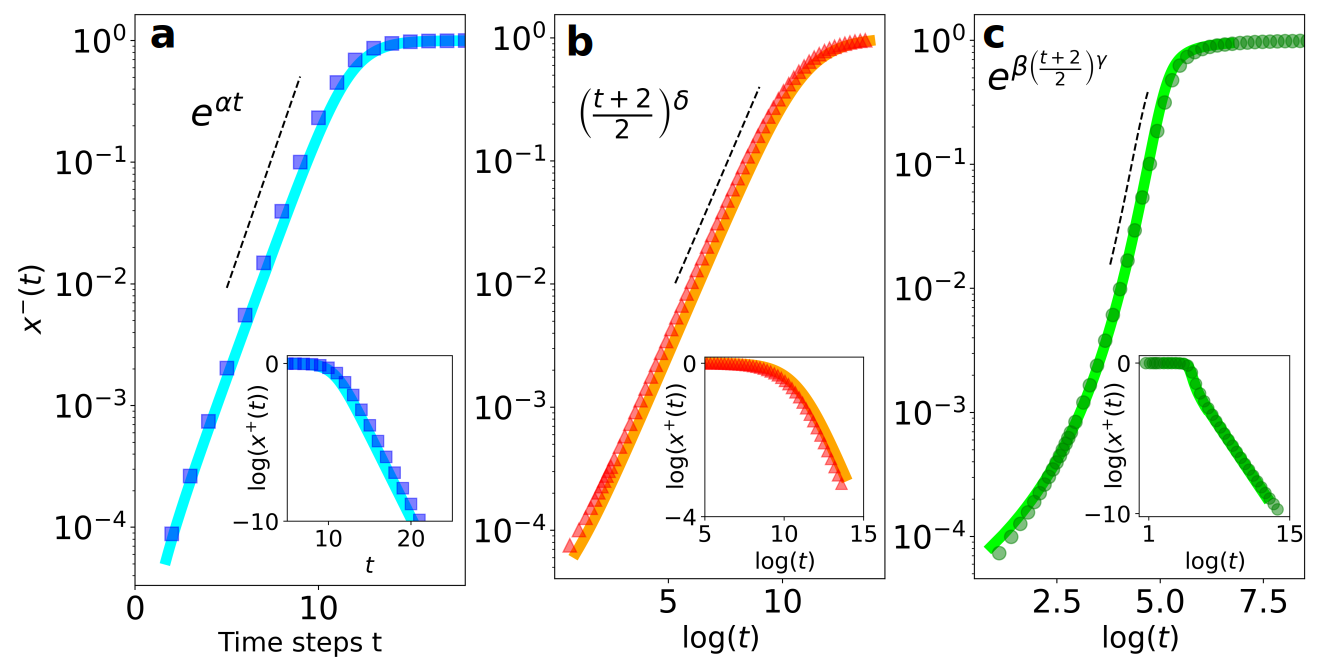
\includegraphics[width=0.7\columnwidth]{Figs/Aging_Threshold/EVO_MOD.pdf}
\caption[Cascade dynamics and fall to the full-adopt state ($x^{-} \sim 1$)]{\label{fig:models} Cascade dynamics and fall to the full-adopt state ($x^{-} \sim 1$) of the Granovetter-Watts model without aging \textbf{(a)} and the versions with endogenous \textbf{(b)} and exogenous \textbf{(c)} aging effects. At (b-c), the evolution is plotted as a function of the logarithm of time $\log{(t)}$ in Monte Carlo steps, as in the insets. The underlying network is a 3-regular random graph and the threshold is $T = 0.2$. The exponent values are $\alpha \simeq 1.0$, $\beta \simeq 1.14$, $\gamma \simeq 0.38$ and $\delta \simeq 1.0$. Numerically integrated solutions of Eq. \eqref{eq:AME_Threshold} (solid lines) describe accurately the numerical results. Monte Carlo simulations are averaged over $M = 5 \times 10^4$ realizations in a network of $N = 1.6 \times 10^5$ nodes.}
\end{figure}

When aging is introduced, the cascade dynamics are much slower than an exponential law (see Fig. \ref{fig:graph_plot}b). For endogenous aging, all non-adopters agents have the same activation probability $p_A(j)$, which decreases at each time step. This gives rise to cascade dynamics well-fitted by a power law increase (see Fig. \ref{fig:models}b),
\begin{equation}
x^{-}(t) \sim x^{-}_0 \, \left( \frac{t + 2}{2}\right)^\delta .
\label{eq:power law}
\end{equation}
For exogenous aging, we observe a slow adoption spread at the beginning followed by a cascade where almost all agents adopt the technology (Fig. \ref{fig:graph_plot}c). This behavior is well-fitted with a stretched exponential increase of the number of adopters (see Fig. \ref{fig:models}c),
\begin{equation}
x^{-}(t) \sim  x^{-}_0\,  e^{\beta \, ((t + 2) / 2)^{\gamma}} .
\label{eq:streched_exp}
\end{equation}
For both aging mechanisms, in the last stages of evolution, a few ``stubborn'' non-adopters remain, although the environment favors the adoption. Due to the chosen activation probability, the number of non-adopters decay with a power law $x^{+}(t) \sim 1/(t+2)$ in both cases (see insets at Fig. \ref{fig:models}(b-c)).

\begin{figure}
\centering \captionsetup{font=sf}
\includegraphics[width=0.6\columnwidth]{Figs/Aging_Threshold/time_steady.pdf}
\caption[Average time to reach the steady state $\tau$]{\label{fig:time_steady} Average time to reach the steady state ($x^{-} > 0.9$) $\tau$ as a function of the system size $N$ for the original Granovetter-Watts model and the versions with endogenous and exogenous aging. The underlying network is a 5-regular random graph and the threshold is $T = 0.12$. Monte Carlo simulations are averaged over $M = 5 \times 10^4$ realizations. Solid lines are the system size-dependent timescale: For the original model, $\tau_{\rm{NO AG.}} = (1/\alpha)\log(N)$, for the endogenous $(\tau_{\rm{ENDO}} = 2N^{1/\delta} - 2)$ and for the exogenous aging ($\tau_{\rm{EXO}} = 2(\log(N)/\beta)^{1/\gamma} - 2$), which follows from the dynamics from Eq. \eqref{eq:exponential}, \eqref{eq:power law} and \eqref{eq:streched_exp}. The exponents $\alpha$, $\beta$, $\gamma$ and $\delta$ are fitted exponents from numerical simulations.}
\end{figure}

Comparing the evolution of the original model with one of the versions with aging, we observe an important separation of time scales. While for the original model, the time to reach the steady state follows a logarithmic increase with the system size, the versions with endogenous and exogenous aging show a power law and a power-logarithmic dependence, respectively (see Fig.\ref{fig:time_steady}). Therefore, the time scale separation between the original model and the versions with aging increases as we increase the system size, and thus, the aging effects are more relevant for large systems.

The power law and the stretched exponential dynamics for endogenous and exogenous aging, respectively, are observed for $z$ and $T$ below the cascade condition ($T < T_c$) and for many different system sizes. This is shown in Fig. \ref{fig:exo_endo_evo} for a random regular, Erd\H{o}s-R\'enyi and  Barab\'asi-Albert networks. In particular, we show that the time-dependent behavior for different system sizes collapses to a single curve when time is scaled with the system size-dependent timescale (previously analyzed in Fig. \ref{fig:time_steady}) that follows from either the power law dynamics $(\tau_{\rm{ENDO}} = 2N^{1/\delta} - 2)$  or the stretched exponential law  $(\tau_{\rm{EXO}} = 2( \log(N)/\beta )^{1/\gamma} - 2)$. Notice that the scaling of the y-axis is necessary for Fig.\ref{fig:exo_endo_evo}(d-f) to show a linear dependence due to the stretched exponential increase.

%d for the different system sizes considering the numerically fitted dependence: stretched exponential for exogenous aging and power law for the endogenous case. Thus, these cascade dynamics are universal for any system size. The variation of parameters $z$ and $T$ only change the exponent values: $\gamma(z,T)$ and $\delta(z,T)$. The exponent dependence is different for graphs with different degree distribution $p_k$. Fig.\ref{fig:exo_endo_evo} shows the particular case for the 3 networks chosen. In particular, for a random-regular graph, the exponents do not depend on the parameter $T$ ($\gamma(z)$ and $\delta(z)$). For the other graphs considered, approaching $T$ to $T_c$ slows cascade dynamics in both cases ($\gamma(z,T)$ and $\delta(z,T)$ decrease). 

A different question is the dependence of the exponents of the power law and stretched exponential with the parameters $z$ and $T$. Numerical results from fitted Monte Carlo simulations for $\alpha(z,T)$, $\delta(z,T)$ and $\gamma(z,T)$ are shown in Figs. \ref{fig:endo_exp} and \ref{fig:exo_exp}. For a random-regular graph, as apparent from Fig. \ref{fig:exo_endo_evo}, the exponents do not depend on the parameter $T$ up to $T_c$ (so the exponents are dependent only on $z$, $\alpha(z)$, $\gamma(z)$ and $\delta(z)$), while for Erd\H{o}s-R\'enyi and Barab\'asi-Albert networks the value of the exponents decrease with $T$ when approaching $T_c$, indicating a slowing down of the dynamics. Also, for these two latter networks, the exponents present a maximum value at a certain value of $z$. This maximum value at a certain $z$ for a fixed $T$ can be understood as being between the two critical lines of Fig. \ref{fig:umbral}.

\subsection{\label{subsec:Approximate master equation and solutions} General mathematical description}

\begin{figure*}
    \centering \captionsetup{font=sf}
    \includegraphics[width=\linewidth]{Figs/Aging_Threshold/FIG_EVO_EXO_ENDO.pdf}
    \caption[Cascade dynamics of the Granovetter-Watts model in graphs]{\label{fig:exo_endo_evo} Cascade dynamics of the Granovetter-Watts model with endogenous (a - c) and exogenous (d - f) aging. From the left column to the right: a random regular graph with degree $z=5$ (a and d), an Erd\H{o}s-R\'enyi graph with average degree $z = 5$ (b and e) and a Barab\'asi-Albert graph with average degree $z = 8$ (c and f). Different colors indicate different values of $T$ and markers correspond to different system sizes: $N = 2,500$ (plus), $10,000$ (circles), $40,000$ (triangles), $160,000$ (crosses) and $640,000$ (squares). Time is scaled according to the system size for each model: $\tau_{\rm{EXO}} = 2(\log(N)/\beta)^{1/\gamma} - 2$, $\tau_{\rm{ENDO}} = 2N^{1/\delta} - 2$, where $\beta$,$\gamma$ and $\delta$ are the fitted exponents from the behavior according to Eq. \eqref{eq:power law} and \eqref{eq:streched_exp}. Solid lines are obtained from the solutions of Eq. \eqref{eq:PA}. Monte Carlo simulations are averaged over $M = 5 \times 10^4$ realizations.}
\end{figure*}

To account for the non-Markovian dynamics introduced by the aging mechanism, we need to go beyond the standard mathematical descriptions of the Granovetter-Watts model \cite{gleeson-2007,gleeson-2008,gleeson-2013}. We do so using a Markovian description by enlarging the number of variables \cite{peralta-2020C,peralta-2020A}. Namely, we classify the agents with degree $k$, number of adopter neighbors $m$ and age $j$ as different sets in a compartmental model in a general framework for binary-state dynamics in complex networks, as described in chapter \ref{ch:Aging in binary state dynamics}. To write down the AME for the Granovetter-Watts model with aging, we need to consider the following possible transitions:
\begin{itemize}
    \item A node $i$, in state $\sigma_i = \pm 1$, changes state and resets internal age with probability $T^{\pm} (k,m,j)$;
    \item A node $i$, in state $\sigma_i = \pm 1$, remains in the same state and resets internal age to zero ($j \to 0$) with probability $R^{\pm} (k,m,j)$;
    \item A node $i$, in state $\sigma_i = \pm 1$, remains in the same state and ages ($j \to j+1$) with probability $A^{\pm} (k,m,j)$.
\end{itemize}
For the specific case of the Granovetter-Watts model, dynamics are monotonic and $T^{-} (k,m,j) = 0$ (no adopter becomes a non-adopter). Moreover, when an agent becomes an adopter, there are neither resetting nor aging events $R^{-} (k,m,j) = A^{-} (k,m,j) = 0$. This means as well that equations for the non-adopters $x^{+}_{k,m,j}$ and adopters $x^{-}_{k,m,j}$ nodes are independent. Thus, we can write the following rate equations for the evolution of the fraction $x^{+}_{k,m,j} (t)$ of $k$-degree non-adopters nodes with $m$ infected neighbors and age $j$:
\begin{align}
\label{eq:AME_Threshold}
\frac{d x^{+}_{k,m,j}}{dt} = & \,  - x^{+}_{k,m,j} - (k-m)\, \beta^s \, x^{+}_{k,m,j} + (k-m+1) \, \beta^s \, x^{+}_{k,m-1,j-1} + A^{+} (k,m,j-1)\, x^{+}_{k,m,j-1},  \\
\frac{d x^{+}_{k,m,0}}{dt}  = & \,   - x^{+}_{k,m,0} - (k - m)\, \beta^s   \,x^{+}_{k,m,0} + \sum_{l = 0} R^{+} (k,m,l)\, x^{+}_{k,m,l}, \nonumber 
\end{align}
where $\beta^s$ is a non-linear function of $x^{+}_{k',m',j'}$ for all values of $k'$,$m'$ and $j'$  (see Eq. \eqref{beta_s}). The remaining step is to define explicitly the transition probabilities for our aging mechanisms. For both exogenous and endogenous aging, the adoption probability is the probability that an agent is activated and has a fraction of adopters that exceeds the threshold $T$, which means that 
\begin{equation}
T^{+}(k,m,j) = p_A(j) \, \theta(m/k - T),
\end{equation} 
where $\theta(\cdot)$ is the Heaviside step function. 

The reset and aging probabilities for endogenous and exogenous aging mechanisms are different. The simplest case is endogenous aging where there is no reset $R^{\pm} (k,m,j) = 0$ and agents increase by one the age with probability 
\begin{equation}
A^{+} (k,m,j) = \,  1 - T^{+}(k,m,j) = \, 1 - p_{A}(j)\, \theta \left( m/k - T \right).
\end{equation}
When aging is exogenous, the reset probability is the probability to activate and not adopt 
\begin{equation}
R^{+} (k,m,j) = p_A (j)\, \left(1 - \theta \left(m/k - T\right)\right). 
\end{equation}
Thus, agents that age are just the ones that do not activate, $A^{+} (k,m,j) = 1 - p_A(j)$.

Using these definitions, we have integrated numerically Eq. \eqref{eq:AME_Threshold} for the Granovetter-Watts model with both endogenous and exogenous aging. Numerical solutions give  good agreement with Monte Carlo simulations (see Fig. \ref{fig:models}). However, in a general network, considering a cutoff for the degree $k = 0,\dots,k_{\rm{max}}$ and age $j = 0,\dots,j_{\rm{max}}$, the number of differential equations to solve is $(k_{\rm{max}} + 1)\, (k_{\rm{max}} + 1)\, (j_{\rm{max}} + 1)$ according to the three subindexes of the variable $x^{+}_{k,m,j}$. This number grows with the largest degree square and largest age considered and thus, some further approximations are needed to obtain a convenient reduced system of differential equations. 

\begin{figure}
    \centering \captionsetup{font=sf}
    \includegraphics[width=0.7\columnwidth]{Figs/Aging_Threshold/ENDO.pdf}
    \caption[Exponent for the Granovetter-Watts model]{\label{fig:endo_exp} Exponent $\alpha$ for the original Granovetter-Watts model (empty markers) and $\delta$ for the version with endogenous aging (filled markers) for different values of the average degree $z$ (and $T = 0.1$) \textbf{(left)} and as a function of $T$ for fixed $z$ \textbf{(right)}. Different markers indicate results from Monte Carlo simulations with different topologies: red triangles indicate an Erd\H{o}s-R\'enyi (ER) graph, blue circles indicate a random regular (RR) graph and green squares indicate a Barab\'asi-Albert (BA) graph. In the right panel, the average degree is fixed $z = 5$ for ER and RR, and $z = 8$ for the BA. Predicted values by Eq. \eqref{eq:alpha} (solid lines) fit the results for each topology. System size is fixed at $N = 4 \times 10^6$ for the original model and $N = 3.2 \times 10^5$ for the version with aging.}
\end{figure}

As an ansatz, we assume that timing interactions can be effectively decoupled from the adoption process so the solution of Eq. \eqref{eq:AME_Threshold} can be written as
\begin{equation}
    \label{eq:assumption1}
    x^{+}_{k,m,j}(t) = x^{+}_{k,m}(t) \, G_{j} (t),
\end{equation}
where $x^{+}_{k,m}$ is the fraction of non-adopters with degree $k$ and $m$ infected neighbors $x^{+}_{k,m} = \sum_{j} x^{+}_{k,m,j}$ and there is an age distribution $G_{j} (t)$, independent of the adoption process.

If we sum over the variable age $j$ in Eq. \eqref{eq:AME_Threshold}, we can rewrite the following rate equations for the variables $x^{+}_{k,m}$
\begin{equation}
    \label{eq:threshold_AME_red}
    \frac{d x^{+}_{k,m}}{dt}  = \,  - \langle p_A \rangle \, \theta(m - kT)\, x^{+}_{k,m} - (k - m) \, \beta^s \,  x^{+}_{k,m} + (k - m + 1)\, \beta^s \,  x^{+}_{k,m-1},
\end{equation}
where aging effects are  just included in $\langle p_A \rangle(t)$: 
\begin{equation}
    \langle p_A \rangle(t) = \sum_{j = 0}^{\infty} p_A(j) \, G_j (t).
\end{equation}

Using the definition of the fraction of $k$-degree adopters $x^{-}_{k} (t)$,
\begin{equation}
    x^{-}_{k}(t) = 1 - \sum_{j=0}^{\infty} \sum_{m = 0}^k x^{+}_{k,m,j},
\end{equation}

and along the lines of Ref. \cite{gleeson-2013}, we use the following ansatz

\begin{equation}
    x^{+}_{k,m} = (1 - x^{-}_{k} (0)) \, B_{k,m}[\phi],
\end{equation}

\begin{figure}
    \centering \captionsetup{font=sf}
    \includegraphics[width=0.7\columnwidth]{Figs/Aging_Threshold/EXO.pdf}
    \caption[Exponent $\gamma$ for the Granovetter-Watts model with exogenous aging]{\label{fig:exo_exp} Exponent $\gamma$ for the Granovetter-Watts model with exogenous aging for different values of the average degree $z$ ($T = 0.1$) \textbf{(left)} and as a function of  $T$ for fixed $z$ \textbf{(right)}. Different markers indicate results from Monte Carlo simulations with different topology: red triangles indicate an Erd\H{o}s-R\'enyi (ER) graph, blue circles indicate a random regular (RR) graph and green squares indicate a Barab\'asi-Albert (BA) graph. In the right panel, the average degree is fixed $z = 5$ for ER and RR, and $z = 8$ for the BA. Predicted values by numerical integration of Eqs. \eqref{eq:PA} (solid lines) fit approximately the results for each topology. System size is fixed at $N = 3.2 \times 10^5$.}
    \end{figure}

where $B_{k,m}[\phi]$ is the binomial distribution with $k$ attempts, $m$ successes and with success probability $\phi$. From this point, we derive from Eq. \eqref{eq:threshold_AME_red} a reduced system of two coupled differential equations for the fraction of adopters $x^{-}(t) = \sum_k p_k x^{-}_{k} (t)$ and an auxiliary variable $\phi (t)$ (see details in Ref. \cite{gleeson-2013}):
\begin{equation}
    \label{eq:PA}
        \frac{d x^{-}}{dt} = \langle p_A \rangle [ h(\phi) - x^{-} ], \quad \quad \frac{d \phi}{dt} = \langle p_A \rangle [ g(\phi) - \phi ],
\end{equation}
where $\phi(t)$ can be understood as the probability that a randomly chosen neighbor of a non-adopter node is an adopter at time $t$. The functions $h(\phi)$ and $g(\phi)$ are nonlinear functions of this variable $\phi$
\begin{align}
    h (\phi)  = & \,  \sum_{k=0}^{\infty} p_k\,  \left( x^{-}_{k} (0) + (1 - x^{-}_{k} (0))\,  \sum_{m = kT}^{k} B_{k,m}[\phi]\right),\nonumber\\
    \\
    g (\phi)  = & \, \sum_{k=0}^{\infty} \frac{k}{z}\,  p_k \,  \left( x^{-}_{k} (0) + (1 - x^{-}_{k} (0)) \, \sum_{m = kT}^{k} B_{k-1,m}[\phi]\right). \nonumber
\end{align}
 When $\langle p_A \rangle$ is replaced by a constant, Eqs. \eqref{eq:PA} reduce to previous results for the original model \cite{gleeson-2008}.
 
Determining the distribution $G_j (t)$ a priori is not easy. For endogenous aging, all non-adopters have the same age at each time step and $G_j (t) = \delta(j-t)$ (where $\delta(\cdot)$ is the Dirac delta function). Therefore, $\langle p_A \rangle = 1/(t+2)$. The numerical solution of Eq. \eqref{eq:PA} gives a good agreement with Monte Carlo simulations (see Fig. \ref{fig:exo_endo_evo}(a-c)). For the case of exogenous aging, the reset of the internal clock makes more difficult a choice for $G_j (t)$.  Inspired on the stretched exponential behavior of $x^{-}(t)$ observed from Monte Carlo simulations, we propose $\langle p_A \rangle = 1/(t+2)^\mu$. For $\mu = 0.75$, the numerical solutions of Eq. \eqref{eq:PA} gives a very good agreement with our Monte Carlo simulations (see Fig. \ref{fig:exo_endo_evo} (d-f)).

\subsection{\label{subsec Analytical results} Analytical results}


To obtain an analytical result for the cascade condition and for the exponents of the predicted exponential, stretched-exponential and power law cascade dynamics that we fitted from Monte Carlo simulations, we need to go a step beyond the numerical solution of our approximated differential equations (Eqs. \eqref{eq:AME_Threshold} and \eqref{eq:PA}). 
%Although the approximate master equation solutions give a good agreement with Monte Carlo simulations, are not able to confirm the cascade condition and the predicted exponential, stretched-exponential and power law cascade dynamics that we fitted from Monte Carlo simulations. We need further approximations to derive analytically the dynamics and the exponent dependence with the control parameters.

%To obtain the cascade condition, we follow the methodology from Ref. \cite{gleeson-2007}. 
For a global cascade to occur, it is needed that the variable $\phi(t)$ grows with time. If we assume a small initial seed ($x^{-}_{k} (0) \; \to \; 0$), Eq. \eqref{eq:PA} can be rewritten as in Ref. \cite{gleeson-2007}
\begin{equation} % Revisar la ecuacion y el papel de k
    \label{eq:pre_lin}
    \frac{d \phi}{dt}  = \langle p_A \rangle \, \left( -\phi + \sum_{k=1}^{\infty} \frac{k}{z} \, p_k \, \sum_{m = k\, T}^{k} B_{k-1,m} [\phi] \right).
\end{equation}
Rewriting the sum term as $\sum_{l=0}^{\infty} C_l \, \phi^l$, with coefficients 
\begin{equation}
    \label{eq:coef_phi}
    C_l = \sum_{k=l}^{\infty} \sum_{m=0}^{l} { k-1 \choose l} \, {l \choose m} \, (-1)^{l+m} \, \frac{k}{z} \, p_k \, \theta\left(m/k - T \right),
\end{equation}
we linearize Eq. \eqref{eq:pre_lin} around $\phi = 0$:
\begin{equation}
    \label{eq:linear}
    \frac{d \phi}{dt} \approx  \langle p_A \rangle \, ( C_1 -1) \, \phi.
\end{equation}
The solution for Eq. \eqref{eq:linear} is then
\begin{equation}
    \label{eq:phi_general}
    \phi(t) = x^{-}_{0}\,  e^{(C_1 - 1) \, \int_0^t \langle p_A \rangle (s) \, ds},
\end{equation}
given that $ \phi(0) = x^{-}_{0}$.

Linearization is useful to determine the time dependence of the cascade process.  Assuming a small initial seed and rewriting the term $h(\phi)$ as  $ \sum_{l=0}^{\infty} K_l\,  \phi^l $, the linearized equation for the fraction of adopters $x^{-}(t)$ becomes
\begin{equation}
    \label{eq:linear_r}
    \frac{d x^{-}}{dt} \approx  \langle p_A \rangle\,  ( K_1 -1)\, \phi,
\end{equation}
where the coefficients $K_l$ are
\begin{equation}
    \label{eq:coef_rho}
    K_l = \sum_{k=l}^{\infty} \sum_{m=0}^{l} { k \choose l} \, {l \choose m} \, (-1)^{l+m}\,  p_k \, \theta\left( m/k - T \right).
\end{equation}

A solution for the fraction of adopters $x^{-}(t)$ can be obtained from  Eqs. \eqref{eq:phi_general} and \eqref{eq:linear_r}.  For the case of the Granovetter-Watts model without aging, setting $\langle p_A \rangle = 1$,  the solution is an exponential cascade dynamics
\begin{equation}
    x^{-}(t) = x^{-}_{0} \, e^{(C_1 - 1)\, t}.
\end{equation}
Therefore, the number of adopters $x^{-} (t)$ follows an exponential increase with exponent $\alpha(z,T)$:
\begin{equation}
    \label{eq:alpha}
    \alpha(z,T) = C_1 - 1 = \sum_{k=0}^{\lfloor 1/T \rfloor} \frac{k \, (k - 1)}{z}\, p_k - 1,
\end{equation}
where $C_1$ is computed from Eq. \eqref{eq:coef_phi}. 

For endogenous aging, the same derivation is valid to determine the exponents $\delta(z,T)$. Using $\langle p_A \rangle = 1/(t+2)$, the fraction of adopters follows a power law dependence,
\begin{equation}
    \label{rho_endo}
    x^{-}(t) = x^{-}_{0} \, \left( \frac{t+2}{2} \right)^{(C_1 - 1)}.
\end{equation}
The exponent reported for the power law cascade dynamics $\delta(z,T)$ turns out to be, therefore, the same exponent as the one for the exponential behavior where there is no aging:  $\delta(z,T)= \alpha(z,T)= C_{1} - 1$. Fig. \ref{fig:endo_exp} compares the prediction of Eq. \eqref{eq:alpha} with the results computed from Monte Carlo simulations. There is a good agreement for both Barab\'asi-Albert and Erd\H{o}s-R\'enyi networks for all values of $T$ and $z$. For a random-regular graph, the predicted dependence, $\alpha(z) = z - 2$, is not a good approximation for large $z$. This is because the presence of small cycles increases importantly in a random-regular graph as the average degree $z$ grows \cite{wormald_1999} and the locally-tree assumption made for the derivation of the rate equations (Eq. \eqref{eq:AME_Threshold}) is not valid anymore. A different approach is necessary for clustered networks (as in Ref.\cite{Leah2022} for the Granovetter-Watts model). 

Moreover, from Eq. \eqref{eq:linear}, we can extract the cascade condition for the Granovetter-Watts model in general. Since $\langle p_A \rangle(t)$ is always positive, global cascades occur when $(C_1 - 1) > 0 $, so the cascade condition is:
\begin{equation}
    \label{eq:umbral}
    T < T_c = \frac{1}{\sum_{k=0}^{\infty} \frac{k \, (k - 1)}{z}\, p_k}.
\end{equation}
This cascade condition does not depend on the aging term $\langle p_A \rangle(t)$ and thus, it is the same as for the Granovetter-Watts model without aging. In Fig. \ref{fig:umbral}, the red solid line is the result of this analytical calculation, and it is in good agreement with the numerical results. 

\begin{figure}
    \centering \captionsetup{font=sf}
    \includegraphics[width=0.5\columnwidth]{Figs/Aging_Threshold/LATT_PLOT.png}
    \caption[Cascade spreading of the Granovetter-Watts model in a lattice]{\label{fig:evo_lat} Cascade spreading of the original Granovetter-Watts model \textbf{(a)} and the versions with exogenous \textbf{(b)} and endogenous \textbf{(c)} aging on a Moore neighborhood lattice with size $N = L \times L$, $L = 405$. Yellow and purple nodes are adopters and non-adopters, respectively. Time increases from left to right. Initial seeds are selected favoring cascades: one agent and all him/her neighbors are set as adopters at the center of the system.}
\end{figure}

For exogenous aging, an analytical expression for the exponent $\gamma(z,T)$ is not obtained following this methodology. Still, we can fit the exponent from the numerical solutions in Fig. \ref{fig:exo_endo_evo} (d-f). Fig.\ref{fig:exo_exp} shows a good comparison between the exponent calculated from the numerical solutions and the one calculated from  Monte Carlo simulations. The dependence of $\gamma(z,T)$ with the parameters $z$ and $T$ is qualitatively similar to the dependence of  $\alpha(z,T)$.

\section{\label{sec:Lattice} Results on a Moore lattice}

The Granovetter-Watts model in a two-dimensional regular lattice with a Moore neighborhood (nearest and next nearest neighbors) has a critical threshold (cascade condition) $T_c = 3/8$ \cite{centola-2007}. Below this value, cascade dynamics follows a power law increase in the density of adopters $x^{-}(t)$, which does not depend on the threshold value $T$ \cite{centola-2007}. In Fig. \ref{fig:evo_lat}a, we show a typical realization of this model: From an initial seed, the adoption radius increases linearly with time until all agents adopt the technology.

When aging is considered, cascade dynamics become much slower and a dependence on $T$ appears. When the aging mechanism is exogenous, Monte Carlo simulations indicate cascade dynamics following a power law $x^{-}(t) \approx t^{\zeta(T)}$. Qualitatively, we observe that while in the case without aging there was a soft interface between adopter and non-adopters, aging causes a strong roughening in the interface and the presence of non-adopters inside the bulk (see Fig. \ref{fig:evo_lat}b). In addition, the exponent values fitted from Monte Carlo simulations allow us to collapse curves for different system sizes (see Fig. \ref{fig:lattice}a). Due to finite size effects, the interface between adopters and non-adopters eventually reaches the borders of the system and the remaining non-adopters, in the bulk, will slowly adopt with the density of adopters following the functional shape $x^{-}(t) = 1- 1/(t+2)$.

Fig.\ref{fig:evo_lat}c shows the dynamics towards global adoption for endogenous aging. In comparison with the case of exogenous aging, we do not observe strong interface roughening between adopters and non-adopters, because non-adopters are not present in the bulk. Monte Carlo simulations indicate a very slow increase of the density of adopters $x^{-}$, similar to a power-logarithmic growth  $x^{-}(t) \approx (\log(t))^{\nu}$, with a threshold dependent exponent $\nu(T)$  (Fig. \ref{fig:lattice}b). Our general approximation used for complex networks assumes a tree-like network, and it is not appropriate for the Moore lattice. 

\begin{figure}
    \centering \captionsetup{font=sf}
    \includegraphics[width=\columnwidth]{Figs/Aging_Threshold/FIGA.pdf}
    \caption[Cascade dynamics snapshots in a lattice]{\label{fig:lattice} Cascade dynamics of the Granovetter-Watts model with exogenous \textbf{(a)} and endogenous \textbf{(b)} aging on a Moore neighborhood lattice. Different colors indicate different values of the threshold $T$. Different markers indicate the results of Monte Carlo simulations with different system size $N = L \times L$:  $L = 50$ (crosses), $100$ (triangles), $200$ (circles) and $400$ (squares). In (a), time is scaled according to size $\tau = L^{2 / \zeta}$. Discontinuous solid lines indicate a power law behavior with exponent $ \zeta = 4/3$ (blue), $1$ (red) and $2/3$ (green). In (b), the system sizes are not scaled due to the slow dynamics. Discontinuous solid lines indicate a power-logarithmic behavior, $x^{-}(t) \, N \sim \log(t)^{\nu} $, with exponent $ \nu = 7/3$ (blue), $2$ (red) and $5/3$ (green).}
\end{figure}
    

\section{\label{sec:Summary and Conclusions} Summary and discussion}

We have addressed in this chapter the role of aging in general models with binary-state agents interacting in a complex network. Temporal activity patterns are incorporated by means of a variable that represents the internal time of each agent. We have developed an approximate Master Equation for this general situation. In this framework, we have explicitly studied the effect of aging in the Granovetter-Watts model as a paradigmatic example of Complex Contagion processes. Aging implies a lower probability to change state when the internal time increases. We considered  two aging mechanisms: endogenous aging, in which the internal time measures the persistence time in the current state, and exogenous aging, in which the internal time measures the time since the last update attempt.

%To summarize, we have explored the effect of exogenous and endogenous aging in a stochastic binary-state model. Autonomous agents have now an internal time counting the persistence time in the same state (or since a reset for the exogenous aging mechanism). We use Threshold model as a paradigmatic example where, even for the original model, one needs to go beyond heterogeneous mean field to have agreement with Monte Carlo simulations.

Our theoretical framework with some approximations to attain analytical results provide a good description of the results from Monte Carlo simulations for Erd\H{o}s-R\'enyi, random-regular and Barab\'asi-Albert networks. For these three types of complex networks, we found that the cascade condition $T_c$ (critical value of the threshold parameter $T$ as a function of mean degree $z$ of the network) for the full spreading from an initial seed is not changed by the aging mechanisms. However, aging modifies in non-trivial ways cascade dynamics of the process. The exponential growth with exponent $\alpha(z,T)$ of the density of adopters in the absence of aging becomes a power law with exponent $\delta(z,T)$ for endogenous aging, and a stretched exponential characterized by an exponent $\gamma(z,T)$ for exogenous aging. We have analyzed the exponents' dependence with the order parameters $\alpha(z,T)$, $\delta(z,T)$, $\gamma(z,T)$ and shown that $\delta(z,T)=\alpha(z,T)$, for which an analytical expression is obtained.

Our general theoretical framework, based on the assumption of a tree-like network, is not appropriate for a regular lattice. In this case, we have been only able to run Monte Carlo simulations. Our results indicate that  exogenous aging gives rise to adoption dynamics characterized by an increase in the interface roughness, by the presence of non-adopters in the bulk, and by a power law growth of  the density of adopters with exponent $\zeta (T)$, while in the absence of aging $\zeta = 2$ independently of $T$. Endogenous aging, on the other hand, produces very slow (logarithmic-like) dynamics, with a threshold-dependent exponent $\nu(T)$.

%In addition, the case of lattice is studied in a separate scheme. When aging is included, a dependence on the threshold parameter of the model $T$ appears naturally. For the exogenous aging, dynamics change to a power law behaviour , with an exponent that depends on $T$, universal for any system size. This aging mechanism also show particular behaviour as interface branching and presence of non-adopters inside the adoption bulk. On the other hand, the endogenous aging shows a very slow adoption increase similar to logarithmic. For large system sizes, to reach the fully-adopted state takes a large number of time steps. Since the dependence on parameter $T$ has a particular shape for both cases, further work would include taking the continuous limit to obtain an analytical derivation of the exponent to compare with Monte Carlo simulations. 

%Our analytical and numerical results show that cascade condition does not change when aging is added to this model. Regarding to cascade dynamics, we show that original model exhibits an exponential increase which becomes slower when aging is added.  Exogenous aging exhibits a stretched exponential increase while endogenous aging shows a power law behaviour. This behaviour has been proven to be universal for different system sizes, networks and control parameter values (uniform threshold $T$ and average degree $z$). Nevertheless, the exponent depends with the topology and the parameters.

%We build an approximate master equation, general for any binary-state model with temporal activity patters. The numerical resolution of the AME shows a very good agreement with Monte Carlo simulations (see Fig.\ref{fig:models}). In particular, for the case of Threshold model with aging, the AME is reduced to a system of only two differential equations when we decouple the age distribution from the adoption process. It is shown that numerical integration also presents a good agreement with Monte Carlo simulations.

%To predict the exponential (from the original model) and power law behaviour (endogenous aging), we linearize the previous system of differential equations. An analytical expression for the exponents is extracted, general for any threshold $T$ and any network (with $p_k$) with average degree $z$ (see Eq.\eqref{eq:alpha}). Exponents from the exogenous aging dynamics are compared with the numerical integration solution of the reduced system of differential equations (Eq. \eqref{eq:PA}).

%Since we focused only on infinite, uncorrelated networks with negligible clustering, we observe that the approximation is not valid for random-regular graphs with high degree. Therefore, a generalization of the AME to networks with high clustering and degree-degree correlations is needed. Moreover, would be interesting a different approach with a pair approximation, including the adoption dependence also to the age distribution. Another approach to binary-state dynamics with timing interactions is consider the stochastic and size effects into the derivation (as in Ref.\cite{peralta-2020B}).

%In addition, the case of lattice is studied in a separate scheme. When aging is included, a dependence on the threshold parameter of the model $T$ appears naturally. For the exogenous aging, dynamics change to a power law behaviour , with an exponent that depends on $T$, universal for any system size. This aging mechanism also show particular behaviour as interface branching and presence of non-adopters inside the adoption bulk. On the other hand, the endogenous aging shows a very slow adoption increase similar to logarithmic. For large system sizes, to reach the fully-adopted state takes a large number of time steps. Since the dependence on parameter $T$ has a particular shape for both cases, further work would include taking the continuous limit to obtain an analytical derivation of the exponent to compare with Monte Carlo simulations. 

This study highlights the importance of non-Markovian dynamics in general  binary-state dynamics and, specifically, in the Granovetter-Watts model. For the problem of innovation adoption that this model addresses, we show how persistence times have an important impact on the adoption cascade. Further work in this direction would be to categorize technologies according to the adoption curve, to show if the system has important resistance to the previous technology (endogenous aging) or a balance between memory and external influence or advertisement (exogenous aging). Furthermore, the theoretical framework presented here gives a basis for further investigations of the memory effects and non-Markovian dynamics in networks, and in particular for  binary-state models with aging. Still, a number of theoretical developments remain open for future work, such as the consideration of stochastic finite size effects \cite{peralta-2020B}, or extending this framework to tri-state models. Also, proper approximations need to be developed to account for some of our numerical results for random-regular networks with high degree, as well as for high clustering, degree-degree correlations networks and for regular lattices, including continuous field equations for this latter case. 


%----------------------------------------------------------------------------------------
%	CHAPTER 3
%----------------------------------------------------------------------------------------
\chapterimage{orange2.png}
\chapterspaceabove{6.75cm}
\chapterspacebelow{7.25cm}

\chapter{Aging effects in the Schelling segreggation model}

The Schelling model has become a paradigm in social sciences to explain the emergence of residential spatial segregation, even in the presence of high tolerance to mixed neighborhoods by the side of citizens. In particular, we consider a noisy constrained version of the Schelling model, in which agents maximize its satisfaction, related to the composition of the local neighborhood, by infinite-range movements towards satisfying vacancies. We add to it an aging effect by making the probability of agents to move inversely proportional to the time they have been satisfied in their present location. This mechanism simulates the development of an emotional attachment to a location where an agent has been satisfied for a while. The introduction of aging has several major impacts on the model statics and dynamics: the phase transition between a segregated and a mixed phase of the original model disappears, and we observe segregated states with a high level of agent satisfaction even for high values of tolerance. In addition, the new segregated phase is dynamically characterized by a slow power-law coarsening process similar to a glassy-like dynamics.

\section{Introduction}

Thomas Schelling introduced a simple segregation model   \cite{schelling-1969,Schelling,schellingbook,hegselmann-2017} in which agents of two colors are distributed randomly on a chess-board, leaving some locations free. Agents are unsatisfied if more than a half of the eight nearest neighbors have different color. Randomly, the unsatisfied agents will move to available satisfying locations of the neighborhood. This model has had a very significant impact for several reasons: The ``hand-made'' simulations performed by T. Schelling by moving pawns on a chessboard are an early precedent of the use of  agent-based simulations in Social Sciences. It is also one of the first social models to show emergent behavior as a result of simple interactions among agents, a characteristic of complex systems. A robust result of the model is that segregation occurs even when individuals have a very mild preference for neighbors of their own type, so collective behavior is not to be understood in terms of individual intentions. In addition, the model introduced the concept of behavioral threshold that inspired a number of other models of collective social behavior \cite{granovetter}. But still currently, Schelling's model is at the basis of fundamental studies of the micro-macro paradigm  in Social Sciences \cite{grauwin-2009}, while it continues to have important implications for social and economic policies addressing the urban segregation problem \cite{clark-1991,Sassen,Clark,lamanna-2018}. A main limitation of the Schelling model is that it has no history or memory by which, for example, residents might prefer to maintain their present location \cite{silver-2021}. In this paper we address this limitation on the effects of memory. 

As a result of the notable implications of this model and the robustness of the emerging segregation, there exists a vast literature around Schelling's results. Many variants of the original Schelling model have been reported modifying the rules that govern the dynamics, the satisfaction condition, or including other mechanisms, network effects, or specific applications \cite{Vinkovic,stauffer-2007,Dall_Asta_2008,gracia-lazaro-2009,Gauvin_2009,Gauvin_2010,domic-2011,henry-2011,unified,Interfacial_roughening,stauffer-2013,lenormand-2015,barmpalias-2018,jensen-2018,holden-2019,sert-2020,agarwal-2020,vieira-2020,ortega-2021,ortega-2021.2}. In particular, the Schelling model has been studied from a Statistical Physics point of view due to its close relation to different forms of Kinetic Ising-like models \cite{stauffer-2007,stauffer-2013}, and also addressing general questions of clustering and domain growth phenomena, as well as for the existence of phase transitions from segregated to non-segregated phases. For example, the relation with phase separation in binary mixtures has been considered \cite{Dall_Asta_2008,Vinkovic}, as well as the connection with the phase diagram of spin-1 Hamiltonians \cite{BEG,BlumeCapel,Gauvin_2009,Gauvin_2010}.
%Moreover, the Schelling model has similarities with various physical models %used to describe phenomena as surface tension or clustering effects. In fact, %Refs. \cite{Dall_Asta_2008,Vinkovic} show relation with binary mixtures in %physics and Ref. \cite{Gauvin_2009} highlight similarities with the phase %diagram of the Blume-Capel model \cite{BlumeCapel}. 
In this context a useful classification of models is to distinguish between two possible types of dynamics \cite{Dall_Asta_2008}: ``constrained'', where agents just move to satisfying vacancies (if possible), and ``unconstrained'',  where agents' motion does not prevent them to remain unsatisfied. In addition, the motion can be short-range (only to neighboring sites, as in the original model) or long-range. Constrained motion has been named ``solid-like'' because it generally leads to frozen small clusters, while unconstrained motion has been considered ``liquid-like'' because it allows for large growing clusters \cite{Vinkovic}. Including the motion of satisfied agents leads to a noisy effect playing the role of temperature in a statistical physics approach. 

It is known that human interactions do not occur at a constant rate. They rather show  a bursty character with a non-Poissonian inter-event time distribution that reflects a memory from past interactions. \cite{barabasi-2005,moro,oriol,rybski-2012,zignani-2016,kumar-2020}
However, most social simulations, including simulations of variants of the Schelling model, implicitly assume a constant rate of interactions or state updating. "Aging" is one form of memory effect on which the rate of interactions depends on the persistence time of an agent in a state, modifying the transition to a different state \cite{fernandez-gracia-2011,perez-2016,boguna-2014}. This concept of aging, or "social inertia" \cite{Stark2008}, constrains the transitions in a way that the longer an agent remains in a given state, the smaller the probability to change it. Aging has been already shown to modify social dynamics very significantly. For example, in opinion dynamics, aging is able to produce coarsening towards a consensus state in the voter model \cite{fernandez-gracia-2011,peralta-2020} or to induce a continuous phase transition in the noisy voter model \cite{artime-2018}. With the motivation of  established relevant effects of aging in opinion dynamics, our goal is to characterize how ``aging'' modifies the segregation dynamics of the Schelling model. In this context, aging must be understood as an emotional/economic attachment to a certain location linked to the persistence time in this location. This attachment balances the memory-less and purely rational considerations of the original model \cite{granovetter-1985}. The aging-induced inertia, which results in resistance to movement, is minimalist modeling of behavior with many different possible causes. Besides the moving out cost due to the housing market fluctuations, aging accounts for the links established with the neighborhood’s public goods, venues, schools, etc, which are known to be highly relevant in this context \cite{wasserman-2001,chetty-2016,silver-2021}. These urban elements are also a major consideration when households locate \cite{denton1995persistence,clark-2002,clark-2003,silver2016scenescapes} and aging also accounts for the memory of this decision.

%Our goal is to characterize how ``aging'' modifies the segregation dynamics of the Schelling model. Aging takes into account how the persistence of an agent in a given state modifies the transition rate to a different state \cite{fernandez-gracia-2011,perez-2016,boguna-2014}. This concept of aging, or inertia \cite{Stark2008}, constrains the transitions in a way that the longer an agent remains in a given state, the smaller is the probability to change it. This rate dependence on the persistence times accounts for the observation that human interactions do not occur at a constant rate. They rather show  a bursty character with a non-Poissonian inter-event time distribution \cite{barabasi-2005,moro,oriol,rybski-2012,zignani-2016,kumar-2020}. However, most social simulations, including simulations of variants of the Schelling model, implicitly assume a constant rate of interactions or state updating. Nevertheless, aging has been already shown to modify social dynamics very significantly. For example, in opinion dynamics, aging is able to produce coarsening towards a consensus state in the voter model \cite{fernandez-gracia-2011,peralta-2020} or to induce a continuous phase transitions in the noisy voter model \cite{artime-2018}. 

In this paper, aging is introduced in the Schelling model by considering that agents are less prone to change their location as they get older in a satisfying place. In other words, aging is introduced giving a smaller probability for  satisfied agents to ``move-out'' the longer they have remained in a satisfying neighborhood. We implement this aging mechanism in the long-range noisy constrained version of the Schelling Model \cite{Gauvin_2009}, for which a detailed phase diagram was reported. We study how this phase diagram is modified by the aging mechanism, finding that aging inhibits a segregated-mixed phase transition. This implies that aging favors segregation, a counter-intuitive result. We also describe the coarsening dynamics in the segregated phase showing that aging gives rise to a slower coarsening that breaks the time-translational invariance.
%and associated autocorrelations \cite{puri-2004}, 
%showing that aging gives rise to a slower coarsening and to a glassy type-dynamics %with breaking of the time-translational invariance.

%To perform a detailed study, we perform a quantitative analysis of computer simulation results, guided by some general principles. This approach has been already performed for complex systems as well as social systems where obtaining analytical results seems out of reach. In particular, we will approach the problem via agent-based modeling, a popular approach nowadays in which we simulate interactions between autonomous agents to see the global emerging outcome.


% Esto no es comun in Sci Reports
%The outline of the paper is as follows. We first introduce the NCSM including aging effects, we describe its numerical implementation and define different measures of segregation. In our results we show the obtained phase diagram and compare it with the case without aging. We also analyze the specific interface properties of the final segregated state. We next report on our findings for the dynamical properties of the model. A last section includes a summary of the main results.

\section{Aging in the Sakoda-Schelling model}

The model considered in this work is a variant of the noisy constrained Schelling model \cite{Gauvin_2009} in which we explicitly include aging effects. For simplicity, we refer to this variant as the Schelling model during the rest of the paper to compare with the model presented here: the Schelling model with aging. For both, the system is established on a $L \times L$ Moore lattice with $8$ neighbors per site and periodic boundary conditions, where agents of two kinds (representing, for instance, wealth levels, race, language, etc) occupy the sites. There are also empty sites (vacancies), where agents can move to, depending on their state and on the vacancy neighborhood. The condition of each site $i$ of the lattice will be described with a variable  $\sigma_i$ that takes three possible values: $\sigma_i = \pm 1$ for the two kinds of agents and $\sigma_i = 0$ for vacancies. In addition, depending on the local environment, agents can be in two states: satisfied or unsatisfied. In our case, agents are satisfied if their neighborhood is constituted by a fraction of unlike agents lower than a fixed homogeneous parameter $T$. Otherwise, they are unsatisfied. Therefore, this control parameter $T$ is a measure of how tolerant the population of the system is. We also need a non-zero vacancy density, $\rho_v > 0$, for agents to change their location. This $\rho_v$ is understood as an extra parameter of the model. The initial configuration is built by randomly distributing the agents ($N_{\rm agents} = L^2 \, (1 - \rho_v)$). We always consider one half of agents of each kind.

In the Schelling model considered, an agent chosen by chance moves to a random satisfying vacancy (if any exists) independently of his/her initial state and of the distance. This process is repeated until the system reaches a stationary state. The movement of unsatisfied agents behaves as a driver for the system dynamics, while the motion of satisfied agents plays the role of noise. When tolerance $T$ becomes larger, more satisfying vacancies are present in the system and the noise consequently increases. 

The aging mechanism in our model is introduced by considering an activation probability of the agents inversely proportional to the time spent at a satisfied location, motivated by the definition for opinion dynamics \cite{artime-2018}. This methodology was proposed to mimic the power-law like inter-event time distributions observed in real-world social systems \cite{barabasi-2005,fernandez-gracia-2011}. If an agent $j$ is initially satisfied in her neighborhood, the internal time is set $\tau_j = 0$. Then, in every time step, a randomly chosen agent $j$ follows different rules depending on whether she is originally satisfied or not. If unsatisfied, $j$ moves to any random satisfying vacancy of the system. Otherwise, she moves to another satisfying vacancy with an activation probability $p_j = 1 / (\tau_j + 2)$. In both cases, if no vacancy has a satisfying neighborhood, the agent $j$ remains in the initial site. As before, these rules are iterated until the system reaches a stationary state (if possible). The time is counted in Monte-Carlo steps; after each Monte-Carlo step, that is after $N_{\rm agents}$ iterations, the internal time increases for all satisfied agents in one unit, $\tau_j \to \tau_j + 1$. Notice that, when an unsatisfied agent becomes satisfied due to the neighbor's motion, an internal time $\tau_j = 0$ is set for that agent. As for the Schelling model, there is a noise effect associated with the motion of satisfied agents. In this case, the intensity of this noise is related not only to the tolerance parameter $T$, but to the presence of aging as well. In fact, aging introduces more constraints to the movements and contributes to decreasing the noise.  

Given the number of neighbors available in the Moore lattice, numerical simulations are only performed for a finite set of meaningful tolerance values: $\{1/8,1/7,1/6, \cdots ,6/7,7/8 \}$. During all our analysis, we focus on the low vacancy density region of the phase diagram. In this region, there is an even smaller number of meaningful $T$ values $\{1/8,2/8,...,7/8\}$, because the majority of agents do not see vacancies in their surroundings.

\section{Segregation coefficient}

Many metrics have been introduced in the literature to discern if the final state is segregated or not \cite{Gauvin_2009,lenormand-2015,randomwalks,urban}. The number of clusters is known to be directly related to the segregation because a high presence of small clusters indicates a mixing between agents. As for the Schelling model\cite{Gauvin_2009}, we compute the following metric related to the second moment of the cluster size distribution:
\begin{equation}
s = \frac{2}{\left(L^{2} \, (1-\rho_v)\right)^{2}} \sum_{\{c\}} n_{c}^{2} ,
\end{equation}
where the index of the sum $c$ runs over all the clusters $\{c\}$ and $n_c$ is the number of agents in the cluster $c$. The average of $s$ over realizations after reaching a stationary state is defined as the segregation coefficient $\langle s \rangle$. This metric is bounded between 0 and 1: $\langle s \rangle \to 1$ if there are only 2 equally-sized clusters, and $\langle s \rangle \to 0$ if the number of clusters tends to the number of agents. The cluster detection is performed using the Hoshen-Kopelman algorithm \cite{HoKo}.

Another metric of segregation is the interface density \cite{Dall_Asta_2008}, defined as the fraction of links connecting agents of different kinds. The calculation is done in two steps: estimating the interface density for each agent $j$, $\rho_j$, and then the average over all the agents $\rho$:

\begin{equation}
    \rho_j = \frac{1}{2} \, \left( 1 - \frac{\sigma_j \,  \sum_{k \in \Omega_j} \sigma_k}{\sum_{k \in \Omega_j} \sigma_k^2 } \right) \quad \rm{and} \quad \rho = \frac{1}{N_{\rm agents}} \sum_{j = 1}^{N_{\rm agents}} \rho_j ,
\end{equation}

where the indices $k$ run over the neighborhood of agent $j$, $\Omega_j$. If an agent $j$ is surrounded only by vacant sites, we define by convention $\rho_j = 0$. Performing a realization average of $\rho$, we obtain the average interface density $\langle \rho \rangle$ in the stationary state is denoted as $\langle\rho_{\rm{st}} \rangle$. The evolution of this metric allows us to study the coarsening process.

\section{Results} 

\subsection{Phase diagram}

To discuss the phase diagram of our model, we focus on the region of parameters with a vacancy density $\rho_v < 50 \%$ to avoid diluted states with a majority of vacancies.
For this region, the Schelling model presents 3 different phases \cite{Gauvin_2009}: frozen, segregated and mixed. For low tolerance values, the system freezes in a disordered state, given that there are no satisfying vacancies for any kind of agent. With increasing tolerance, the system undergoes a transition toward a segregated state, which is characterized by a 2-clusters dynamical final state. Finally, for high values of $T$, after another transition, we find a dynamical disordered (mixed) state, in which a vast majority of vacancies are satisfying for both kinds of agents, and small clusters are continuously created and annihilated.

\begin{figure}
\centering \captionsetup{font=sf}
\includegraphics[width=0.85\linewidth]{Figs/Aging_Schelling/fig1.pdf} 
\caption[Average interface density and segregation coefficient]{Average interface density $\langle\rho_{\rm{st}} \rangle$ (\textbf{a}) and segregation coefficient $\langle s \rangle$ (\textbf{b}) at the stationary regime as a function of the tolerance parameter $T$ for two values of the vacancy density $\rho_{v} = 0.5\%$ and $15\%$. Results are shown for both the Schelling model and the variant with aging introduced in this paper. Simulations are performed on an $80\times 80$ lattice and averaged over $5 \cdot 10^{4}$ realizations.}
\label{Fig1}
\end{figure}

These three phases are characterized by measuring the segregation coefficient $\langle s \rangle$ and the average interface density $\langle\rho_{\rm{st}} \rangle$ at the final state. The results for the original model are depicted as a function of the tolerance $T$ in Fig. \ref{Fig1}a for the interface density and in Fig. \ref{Fig1}b for the segregation coefficient. At low values of T, both indicators show a disordered state that falls in the frozen phase.  We also observe a dependence of the transition point with the vacancy density. On the other hand, for high $T$ values, the transition point between segregated and mixed states has no dependence on the parameter $\rho_v$. Notice that mixed and frozen states present a very similar value of $\langle s \rangle$ but can be differentiated by the stationary value of the average interface density $\langle\rho_{\rm{st}} \rangle$. These results are in agreement with the results reported for the Schelling model\cite{Gauvin_2009}, with the extra information provided by the average interface density.

The first quite dramatic effect of including aging in the system is the disappearance of the mixed state from the phase diagram. In both metrics, the difference between the models with and without aging is clearly manifested. For low $T$ values, the frozen-segregated transition behaves similarly to the original model since aging has no implications as the system gets quickly frozen. Nevertheless, for high values of the tolerance $T> 0.5$, the segregated-mixed transition disappears, and the segregated phase is always present. This is not an intuitive effect and one would think that aging, contributing to difficult agent's mobility, should prevent the system from forming fully developed segregated clusters. However, it is just the opposite, and it favors cluster emergence. 

\subsection{Segregated phase: final state}

To gain further insights into the differences in the system dynamics that lead to the extended segregated phase, we compute the fraction of unsatisfied agents at the stationary regime $n_u$ (see Fig. \ref{Fig2}a). This metric plays a role as a marker for the frozen-segregated transition, as shown for the 1D Schelling model \cite{Dall_Asta_2008}. The frozen phase presents a big majority of unsatisfied agents for both models. After the transition, this parameter decays to very low values in the segregated phase, where a majority of agents are satisfied. In this phase, we observe a step-like increasing behavior of the unsatisfied agents with $T$. As the tolerance grows, the number of satisfying vacancies increases and the noisy movement of satisfied agents drives the system evolution, creating eventual unsatisfied agents in the sites that they abandon or target. However, in the Schelling model, the transition to a mixed state at $T = 0.75$ inhibits the creation of clear fronts between agents of different kinds, and it is also associated to a sharp increase of $n_u \simeq 0.05 $ (red squares in Fig. \ref{Fig2}a). The Schelling model with aging, on the other hand, shows a lower fraction of unsatisfied agents during all values of the tolerance above the frozen-segregated transition (blue triangles in Fig. \ref{Fig2}a). So much so, that many realizations reach $n_u = 0$ and this causes the large error bars in Fig. \ref{Fig2}a after the transition. In a counterintuitive way, the introduction of aging causes a higher global satisfaction when compared with the original model in both the segregated and the mixed phases.

The creation of new unsatisfied agents at the final stationary state occurs at the interface between the segregated agent kinds. This is why we study the interface roughness (perimeter) $P$ as a function of the tolerance parameter. To compute this measure, we compute the number of agents of one kind in contact with different kind agents. To perform this calculation, we smooth the interface by considering vacancies surrounded by a majority of agents of a certain kind as members of that kind. In our system of $L \times L$ with periodic boundary, the minimum interface size (perimeter) $P$ between clusters of agents of different kind is $P = 2 \, L$. To avoid the $L$ dependency, we calculate an adimensional magnitude $P/\sqrt{S}$, where $S$ is the number of agents of each kind $S = N_{\rm{agents}}/2 = L^2 \, (1 - \rho_v )/2 $ (surface). This metric $P/\sqrt{S}$ is computed starting from a flat interface as an initial condition and evolving it for $t_{\rm{max}} = 10^4$ MC steps to reach well within the stationary state. With the metric $P/\sqrt{S}$, we are able to estimate how close is the final state interface of our system to the flat interface ($P/\sqrt{S} = 2 \, \sqrt{2}$). The results show an increasing dependence of roughness with the tolerance parameter $T$ (see Fig. \ref{Fig2}b). This growth can be explained as an increase in tolerance means that agents are satisfied with fewer ``same-kind'' neighbors. Therefore, the interface is able to be rougher, keeping the agents in a satisfied state. In addition, notice that all values with different $L$ collapse, so the dependence on the system size has been eliminated. 

\begin{figure}
\centering \captionsetup{font=sf}
\includegraphics[width=\linewidth]{Figs/Aging_Schelling/fig7.pdf} 
\caption[Fraction of unsatisfied agents and roughness]{ (\textbf{a}) Fraction of unsatisfied agents $n_u$ at the stationary regime as a function of the tolerance parameter $T$. (\textbf{b}) Measure of the interface roughness between clusters of different kind of agents at the final stationary state $P/\sqrt{S}$ as a function of the tolerance parameter $T$. Different markers indicate different system sizes: $L = 40$ (circles), $60$ (squares), $80$ (triangles) and $100$ (crosses). Results are shown for both the Schelling model with and without aging. Numerical simulations are performed for $\rho_v = 0.5\%$ and averaged over $5 \cdot 10^4$ realizations. The frozen-segregated transition (dashed black line) and the segregated-mixed transition (gray dot-dashed line) are highlighted to differentiate the phases that the Schelling model exhibits. There are no values of $P/\sqrt{S}$ for the Schelling model above $T = 3/4$ because the segregated-mixed transition occurs. (\textbf{c}) Final state interface zoom snapshot for $T = 0.57$ using the original model. (\textbf{d}) Final state interface zoom snapshot for $T = 0.57$ using the model with aging.  (\textbf{e}) Same as c for $T = 0.86$.}
\label{Fig2}
\end{figure}

Comparing both models, one observes a lower interface roughness for the Schelling model with aging, regardless of the value of $T$. The closest value to the flat interface occurs for the first values of $T$ after the frozen-segregated phase transition (shown in Fig. \ref{Fig2}d). In the original model, we observe higher values of $P/\sqrt{S}$ due to the noise produced by the satisfied agents' behavior (see Fig. \ref{Fig2}c). Moreover, aging allows us to obtain a segregated phase with even larger interface roughness than the maximum observed in the original model for large values of $T$ (see Fig. \ref{Fig2}e). We remark that, when aging is introduced, agents try to join those of their own kind but are less and less prone to change location as time passes. Thus, in the Schelling model with aging, agents in the bulk of the clusters mainly do not move and those moving more often are located at the interface between agent kinds. At medium and large scales, this phenomenon leads to ergodicity breaking in the final state dynamics.

\subsection{Segregated phase: coarsening dynamics}

\begin{figure}
\centering \captionsetup{font=sf}
\includegraphics[width=\linewidth]{Figs/Aging_Schelling/Fig3.pdf} 
\caption[Average interface density evolution]{Average interface density $\langle \rho (t) \rangle$ as a function of time steps for different values of the tolerance parameter $T$ using the Schelling model (\textbf{a}) and the version with aging (\textbf{b}). Average performed over $5 \cdot 10^3$ realizations. Fitted power-law in a black dashed line highlighting the estimated exponent value. We set system size $L = 200$ and $\rho_v = 0.005$.}
\label{Fig3}
\end{figure}

Diverse versions of the original Schelling Model exhibit different behaviors in terms of coarsening dynamics. Recent publications report a power-law like domain growth \cite{Dall_Asta_2008,Interfacial_roughening}. We monitor here the evolution of the interface density $\langle \rho (t) \rangle$, which decreases as $ \langle \rho (t) \rangle \sim t^{-\alpha}$ so the domains should grow in our model following a power-law with time. 

The coarsening process of the Schelling model at the segregated phase ($0.5 \le T < 0.75$) is displayed in Fig. \ref{Fig3}a and Fig. \ref{Fig4}. We find that the average interface density follows a power-law decay with an exponent $\alpha \simeq 0.5$ for the limit of small vacancy density $\rho_v \to 0$, in agreement with the value reported for close variants of the Schelling model \cite{Dall_Asta_2008}. This exponent value is curious since the coarsening in the presence of a conserved quantity (but with local interactions) exhibits an exponent $\alpha = 1/3$ \cite{Maxi}. Nevertheless, the interactions in this model are not local, and the coarsening exponent is more similar to the one in systems with a non-conserved order-parameter ($\alpha = 1/2$). Fig. \ref{Fig3}a shows as well how coarsening changes with the tolerance parameter. Even though the exponent $\alpha$ does not depend on $T$, we observe a certain delay when increasing $T$ from $0.6$ to $0.62$. In the system evolution of Fig. \ref{Fig4}, one can see how the behavior of the satisfied agents for higher tolerance values is translated into rougher interfaces, causing such delay. For $T > 0.75$, the system exhibits a transition towards a mixed state where the interface density fluctuates around $\rho = 0.5$, indicating that the state is constantly disordered.

\begin{figure}
\centering \captionsetup{font=sf}
\includegraphics[width=0.9\linewidth]{Figs/Aging_Schelling/Fig4.pdf} 
\caption[Coarsening towards the segregated state]{Coarsening towards the segregated state at two different values of $T$ for both models. Snapshots are taken for $5$, $500$, $5000$ and $50000$ time steps ordered from left to right. We set system size $L = 200$ and $\rho_v = 0.005$.}
\label{Fig4}
\end{figure}

%, which corresponds with a typical length of clusters growing as $t^{1/z}$ with $z = 2$, the same behaviour as systems with non conserved order-parameter \cite{Bray}.Nevertheless, as the number of agents of each kind is always the same, the analogous to the magnetization of our system is conserved. This exponent is also found in literature for other variants of Schelling model justified by the constrained 1d behaviour, which can be related with the domain growth scaling of a diffusion-limited annihilation problem where for $\rho_v \to 0$, the exponent $\alpha = 1/2$ for the interface density appears naturally \cite{Dall_Asta_2008}.

The Schelling model with aging shows very different behavior (Fig. \ref{Fig3}b). As predicted by the phase diagram, the average interface density exhibits a power-law decay with time for all values of the tolerance $T$ after the frozen-segregated transition. Still, the decay is slower than for the Schelling model, with $\langle \rho (t)\rangle \; \sim \; t^{-0.2}$. A mechanism that could be behind this behavior is that the model with aging counts more satisfied agents than the original model, and their probability to move becomes lower as time goes by. Moreover, satisfied agents inside a cluster will not move and the dynamics in the model take place at the interface. It is, therefore, more difficult for separated clusters to collide and merge, an effect that slows down the decay of the interface density. The persistence of small clusters becomes clear when the snapshots' evolution is compared for both models at the same tolerance value $T = 0.71$ (see Fig. \ref{Fig4}). Moreover, while for the original model the initial clustering for $t = 500$ steps does not determine the final state, in the case of aging the bigger clusters present at the beginning of the evolution are the ones that keep growing, determining the shape of the system configuration after $50000$ time steps. This is a dynamical effect, because the system in both cases tends to a final configuration with 2-clusters.

In the case of the Schelling model with aging, we observe an early cross-over in the dynamics (Fig. \ref{Fig3}b). For $T < 0.75$, the coarsening starts with an initial decay of $\langle \rho (t)\rangle$ faster than $t^{-0.2}$. This occurs because in this regime it is necessary sometimes for the aging effects to become relevant, and initially the system behaves as in the original model. Similarly, for $T \ge 0.75$, $\langle \rho (t)\rangle$ decays slowly for a moment before reaching the power-law behavior for large $t$ values.  Confirming this scenario, Fig. \ref{Fig4} shows that for $T = 0.86$, the system starts evolving similarly to a mixed state until some clusters are created. At this moment, aging prevents the clusters' desegregation, leading the system very slowly to coarsening dynamics and, eventually, to a fully segregated state. 

Regarding the relaxation time to the final state, we see in Fig. \ref{Fig4} how for $T = 0.71$, the stationary state of the Schelling model is reached after approximately $t = 5000$ time steps. In contrast, the version with aging needs much more than $50000$ steps to attain it. This highlights the important temporal  difference between both models in terms of domain growth dynamics, which strongly increases the computational cost of the study of the stationary state of the model with aging. We have been thus able to study only medium and small system sizes in this final regime (see videos included as Supplementary Information S1 and S2).

The dynamics studied thus far are performed considering the limit $\rho_v \to 0$, but the analysis can be extended to higher vacancy densities. For the particular case of high $\rho_v$ and low $T$, aging leads to the formation of a vacancy cluster at the interface between domains (see details in Supplementary information S3).

\subsection{Aging breaks the asymptotic time-translational invariance}

Here, we explore further time translational invariance (TTI) in the model dynamics. For this, we start by defining the two-time autocorrelation function $C(\tau,t_{\rm{w}})$ \cite{spinglassbook} as

\begin{equation}
    C(\tau,t_{\rm{w}}) = \left\langle \frac{1}{M} \, \sum_{i = 1}^{N}  \sigma_i (t_{\rm{w}} + \tau) \,  \sigma_i(t_{\rm{w}}) \right\rangle ,
\end{equation}
where $N$ is the system size,  $\langle \cdot \rangle$ refers to averages over realizations, $t_{\rm{w}}$ is the waiting time to start the autocorrelation measurements, $\tau$ a time interval after $t_{\rm{w}}$ and $M$ is a normalization factor defined as
\begin{equation}
M =  \sum_{i = 1}^{N}  (\sigma_i (t_{\rm{w}} + \tau) \, \sigma_i(t_{\rm{w}}))^2 . 
\end{equation}
which is computed at each realization. 

The autocorrelation function is displayed for the Schelling model with $T = 0.75$ in Fig. \ref{Fig5}a. We observe the curves decreasing with $\tau$ as expected, and that after a characteristic time period ($t_{\rm{w}}^* \approx 5000$ for a system size of $80\times 80$) they collapse into a single curve. This is the regime in which the dynamics becomes TTI, implying that the autocorrelation function does not depend any more on the waiting time, $C(\tau,t_{\rm{w}}) = C(\tau)$ for $ t_{\rm{w}} > t_{\rm{w}}^{*}$. 

\begin{figure}
\centering \captionsetup{font=sf}
\includegraphics[width=\linewidth]{Figs/Aging_Schelling/fig5new.pdf} 
\caption[Two-times autocorrelation]{Two-times autocorrelation $C (\tau,t_{\rm{w}})$ as a function of the time period passed since the waiting time $t_{\rm{w}}$. First, the autocorrelation is shown for the Schelling model at $T = 0.71$ in \textbf{a}, and for the version with aging at $T = 0.71$ in \textbf{b} and $T = 0.86$ in \textbf{c}. The insets are the result of the collapse using $u(\tau,t_w) = \tau/t_w$ (\textbf{b}) and $u(\tau,t_w) = \log(\tau+t_w)/\log(t_w) - 1$ (\textbf{c}). The curves correspond to different values of the waiting time $t_{\rm{w}}$. Calculations performed on a $100 \times 100$ lattice averaged over $5 \cdot 10^{4}$ realizations.}
\label{Fig5}
\end{figure}

For the Schelling model with aging, the dynamics show some different features (Figs. \ref{Fig5}b and \ref{Fig5}c). First, the autocorrelation functions decay slower with $\tau$ in all the cases, which is connected to the long-lived small clusters mentioned previously. We do not find in the simulations any value of $t_{\rm{w}}^*$ for the systems to fall into a TTI regime. Not only that, but a scaling relation including both $\tau$ and $t_{\rm{w}}$ can be applied to collapse the autocorrelation curves (see insets Figs. \ref{Fig5}b and \ref{Fig5}c). This behavior is similar to glassy systems \cite{spinglassbook}, therefore it is useful to use the mathematical description for those systems in our case. In this type of dynamics, a final stationary state is not attainable in the thermodynamic limit, and it is possible to decompose the autocorrelation function into an equilibrium part and an ``aging'' part (aging in the sense of non-equilibrium dynamics in glassy systems)  \cite{spinglassbook,Heisemberg}:

\begin{equation}
    C (\tau, t_{\rm{w}}) \simeq C_{\rm{eq}}(\tau) \; C_{\rm{aging}} u(\tau,t_w) = C_{\rm{eq}}(\tau) \; C_{\rm{aging}} \left( \frac{h (\tau) }{h(t_{\rm{w}})} \right),
\end{equation}

where $C_{\rm{eq}}$ describes the fast relaxation of the system components within each domain (TTI term), $C_{\rm{aging}}$ is a scaling function and $u(\tau,t_w)$ is a normalization factor which, in some cases, can be written as the quotient of an unknown function $h(t)$ at the two times $\tau$ and $t_{\rm{w}}$. This function $h(t)$ is known to be related to the dynamical correlation length  \cite{Heisemberg,8Heisemberg}. In our case, we use $h(t) = t$ to scale the results in Fig. \ref{Fig5}b (see inset). This scaling is valid for values of $T \in [0.5,0.75)$. Nevertheless, higher values of $T$ do not hold a linear scaling, and we need to turn to other functional forms as the normalization factor $u(\tau,t_w) =  \log(\tau+t_w)/\log(t_w) - 1$ used in  Fig. \ref{Fig5}c. This indicates that for $T > 0.75$, the dynamical correlation length evolves in a different and slower way.

\section{\label{sec:Summary and Conclusions} Summary and discussion}

We have studied the effect of aging on a stochastic Threshold model, which combines long-range mobility with local short-range interactions. Specifically, taking as basis the noisy constrained Schelling model, we assign to the agents an internal clock counting the time spent in the same satisfying location. The probability of changing state decreases then inversely proportional to this time. Therefore,  older satisfied agents are less prone to update resident locations. The original model displays a transition between a segregated phase and a mixed one as the tolerance control parameter $T$ increases. This transition disappears when aging is introduced into the system, the mixed phase is replaced by a segregated phase even for high values of the tolerance parameter $T$. As a result, the model with aging presents a higher global satisfaction than without this effect for all values of the tolerance. 

On the dynamical perspective, the relaxation towards the segregated phase features a coarsening phenomena characterized by a power-law decay of the average interface density with time $\langle \rho \rangle \sim t^{-\alpha}$. For the original model in the limit of low vacancy density, the exponent is around $\alpha = 1/2$. This exponent is also reported in other variants of the Schelling model \cite{Dall_Asta_2008,Interfacial_roughening}. Aging gives rise to long-lived small clusters and a slower coarsening, reducing the exponent to $\alpha \simeq 0.2$. We investigated the autocorrelation functions in the segregated phase and found that aging breaks the asymptotic time-translational invariance of the dynamics. This result, along with a nontrivial scaling of the autocorrelation functions, establish close similarities with low-coarsening systems, such as glassy systems, and our Schelling model with aging for high values of the tolerance parameter. Moreover, this work studies the case for equal size populations ignores effects arising from the competition between different population sizes. Further work would be to study a joint effect of minority population and aging.

As for the implications of our results from a social perspective, we must note that the fact that aging favors segregation, inhibiting the segregation-mixed phase transition, is rather counter-intuitive, but gives support to the argument that segregation is a stochastically stable state and may prevail in an all-integrationist world \cite{Zhang}. Our model predicts the appearance of segregation even for tolerance  values close to one. Additionally, the model relaxation time multiplies manifold, which implies that if aging is present the natural state of this system seems to be generically out of equilibrium.   

%----------------------------------------------------------------------------------------
%	CHAPTER 4
%----------------------------------------------------------------------------------------
\chapterimage{orange3.png}
\chapterspaceabove{6.75cm}
\chapterspacebelow{7.25cm}

\chapter{Ordering dynamics and aging in the Symmetrical Threshold model}

The so-called Granovetter-Watts model was introduced to capture a situation in which the adoption of new ideas or technologies requires a certain redundancy in the social environment of each agent to take effect. This model has become a paradigm for complex contagion. Here we investigate a symmetric version of the model: agents may be in two states that can spread equally through the system via complex contagion. We find three possible phases: a mixed one (dynamically active disordered state), an ordered one, and a heterogeneous frozen phase. These phases exist for several configurations of the contact network. Then, we consider the effect of introducing aging as a non-Markovian mechanism in the model, where agents become increasingly resistant to change their state the longer they remain in it.  We show that when aging is present, the mixed phase is replaced, for sparse networks, by a new phase with different dynamical properties. This new phase is characterized by an initial disordering stage followed by a slow ordering process towards a fully ordered absorbing state. In the ordered phase, aging modifies the dynamical properties. For random contact networks, we develop a theoretical description based on an Approximate Master Equation that describes with good accuracy the results of numerical simulations for the model with and without aging.
	
\section{\label{sec:Introduction} Introduction}
	
In recent decades, various techniques of probability and statistical physics have been employed to measure and explain social phenomena \cite{castellano2009statistical,jusup2022social,bianconi2023complex}. A variety of social collective phenomena can be well understood through stochastic binary-state models of interacting agents. In these models, each agent is assumed to be in one of two possible states, such as susceptible/infected, adopters/non-adopters, etc., depending on the context of the model. The interaction among agents is determined by the underlying contact network and the dynamical rules of the model. There are various examples of binary-state models, including processes of opinion formation \cite{Voter-original, sood-2005, Suchecki-2005, fernandez-gracia-2014, redner-2019} and disease or social contagion \cite{granovetter-1978, pastor-satorras-2015}, among others. The consensus problem consists of determining under which circumstances the agents end up sharing the same state or when the coexistence of both states prevails. This is characterized by a phase diagram that provides the boundaries separating domains of different behaviors in the control parameter space. Macroscopic descriptions of these models in terms of mean-field, pair, and higher-order approximations are well established \cite{gleeson-2011}. 
	
An important category of binary-state models are threshold models \cite{watts-2002}, which were originally introduced by M. Granovetter \cite{granovetter-1978} to address problems of social contagion such as rumor propagation, innovation adoption, riot participation, etc. Multiple exposures, or group interaction, are necessary in these models to update the current state, a characteristic of complex contagion models \cite{centola-2007,unknown-author-2018}. The threshold model presents a discontinuous phase transition from a ``global cascade'' phase to a ``no cascade'' phase, which was analyzed in detail in Ref. \cite{watts-2002}. This model has been extensively studied on various network topologies, such as regular lattices, small-world \cite{centola-2007}, random \cite{gleeson-2007}, clustered \cite{hackett-2011,hackett-2013}, modular \cite{gleeson-2008}, hypergraphs \cite{de-arruda-2020}, homophilic \cite{diaz-diaz-2022} and coevolving \cite{min2023threshold} networks. 
	
A main difference between the threshold model and other binary-state models, such as the Voter \cite{Voter-original}, majority vote (MV) \cite{de1992isotropic,pereira2005majority,campos2003small}, and nonlinear Voter model \cite{castellano-2009,mobilia2015nonlinear,mellor2016characterization,Min-2017,jewski-2017,peralta-2018}, is the lack of symmetry between the two states. In the threshold model, changing state is only possible in one direction, representing the adoption forever of a new state that initially starts in a small minority of agents. A symmetric version of the threshold model, with possible changes of states in both directions, was introduced in Refs. \cite{nowak2019homogeneous,nowak2020symmetrical} to investigate the impact of noise and anticonformity. However, a complete characterization of the Symmetrical Threshold model and its ordering dynamics have not been addressed so far.

\section{\label{Symmetrical Threshold model} Symmetrical Threshold model}

%The interaction dynamics of the Symmetrical Threshold model are motivated by the threshold model introduced by M. Granovetter \cite{granovetter-1973}. While the original binary-state model only considers the propagation of one state through the system (asymmetric model), in this study we consider the symmetric case, where both states are allowed to propagate. 
The system consists of a set of $N$ agents located at the nodes of a network. The variable describing the state of each agent $i$ takes one of the two possible values: $s_i = \pm 1$. Every agent has assigned a fixed threshold $0 \leq T \leq 1$, which determines the fraction of different neighbors required to change state. Even though this value might be agent-dependent, we will consider here only the case with a homogeneous $T$ value for all the agents of the system. In each update attempt, an agent $i$ (called active agent) is randomly selected, and if the fraction of neighbors with a different state is larger than the threshold $T$, the active agent changes state $s_i \to -s_i$. In other words, if $m$ is the number of neighbors in state $-1$ out of the total number of neighbors $k$, the condition to change is $\theta(m/k - T)$, for a node in state $+1$, and $\theta((k-m)/k - T)$, for a node in state $-1$, where $\theta(x)$ is the Heaviside step function. Notice that this update rule is equivalent to ``shifted'' Glauber dynamics \cite{glauber1963time}, with swapping probability $1/(1+\exp[\beta(\Delta E + C)]$ (where $\beta$ is the inverse temperature, $\Delta E$ the energy loss to swap the state of a node according to Ising Hamiltonian and $C$ a shifting constant), at the limit of zero temperature ($\beta \to \infty$). We analyze the model dynamics using numerical simulations. Simulation time is measured in Monte Carlo (MC) steps, i.e., $N$ update attempts. Numerical simulations run until the system reaches a frozen configuration (absorbing state) or until the average magnetization, $m = (1/N) \sum_i s_i$, fluctuates around a constant value.

\subsection{Mean-field}

\begin{figure}[t]
	\centering
	\includegraphics[width=0.9\textwidth]{Figs/Aging_STM/FIG1.pdf}
	\caption{\textbf{Phases of the Symmetrical Threshold model.} (a) Phase diagram of the Symmetrical Threshold model in a Complete graph of $N = 2500$ nodes. Dotted and dashed lines correspond to $T = (1-|m_0|)/2$ and $T = (1+|m_0|)/2$, respectively. Average performed over 5000 realizations. (b) Potential representation from Eq. (\ref{eq:potential}) for a set of values of the threshold $T$, shown in different colors.}
	\label{COM_LAT_PD}
\end{figure}

We first consider the mean-field case of the complete graph (all-to-all connections). We take an initial random configuration with magnetization $m_0$ and run numerical simulations for various values of $T$ to construct the phase diagram (shown in Fig. \ref{COM_LAT_PD}a). We find three different phases based on the final state:
\pagebreak
\begin{itemize}
	\item \textbf{Phase I or Mixed}: The system reaches an active disordered state (final magnetization $m_f = 0$) where the agents change their state continuously;
	\item \textbf{Phase II or Ordered}: The system reaches the ordered absorbing states ($m_f = \pm 1$) according to the initial magnetization $m_0$;
	\item \textbf{Phase III or Frozen}: The system freezes at the initial random state $m_f = m_0$.
\end{itemize}

For a given initial magnetization $m_0 \neq 0$ and increasing $T$, the system undergoes a mixed-ordered transition at a critical threshold $T_{c} = (1-|m_0|)/2$, and an ordered-frozen transition at a critical threshold $T_{c}^{*} = (1 + |m_0|)/2 > T_{c}$ (indicated by dotted and dashed black lines in Fig. \ref{COM_LAT_PD}a, respectively). In this mean-field scheme, if the fraction of nodes in state $+1$ is denoted by $x$, the condition for a node in state $-1$ to change its state is given by $\theta(x - T)$, where  $\theta$ is the Heaviside step function. Thus, in the thermodynamic limit ($N\to \infty$), the variable $x$ evolves over time according to the following mean-field equation:<
\begin{equation}
	\frac{dx}{dt} = (1 - x) \; \theta(x - T) - x \; \theta(1 - x - T) = - \frac{\partial V(x)}{\partial x}.
\end{equation}
Here, $V(x)$ is the potential function. The stationary value of $x$, $x_{\rm st}$, is the solution of the implicit equation resulting from setting the time derivative equal to $0$. The stationary solutions are $x_{\rm st} = 1/2$ ($m =0$), the absorbing states $x_{\rm st} = 0,1$ ($m = \pm 1$) or a degenerate continuum of solutions. The stability of these solutions can be understood in terms of the potential $V(x)$:
\begin{eqnarray}
	\label{eq:pot}
	V(x) &=-\int (1 - x) \; \theta(x - T) - x \; \theta(1 - x - T) \; dx \nonumber\\
	&=\frac{x^2}{2} + \frac{1}{2} \left( T^2 - 2T - x^2 + 1\right) \; \theta(T+x-1)\\
	&- \frac{1}{2} \left( T^2 - 2T - x(x-2)\right) \; \theta(x - T)\nonumber
\end{eqnarray}
The minimum and maximum values of $V(x)$ correspond to stable and unstable solutions, respectively. Figure \ref{COM_LAT_PD}b shows the potential's dependence on the magnetization, obtained after a variable change $m = 2x-1$ in Eq. (\ref{eq:pot}). For $T < 0.5$, $m = 0$ is a stable solution, but increasing the threshold reduces the range of values of the initial magnetization from which this solution is reached, enclosing Phase I between the unstable solutions $m = 1-2\, T$ and $2\, T-1$. In fact, if $m_0 > 1-2\, T$, the system reaches the absorbing solution $m=+1$, while if $m_0 < -1+2\, T$, it reaches $m=-1$ (Phase II). For $T = 0.5$, there is just one unstable solution at $m=0$, and all the initial magnetization values reach the absorbing states $m=\pm 1$. For $T > 0.5$, the potential is equal to a constant value for a range of $m_0$, which means that an initial condition will remain in this state forever (Phase III). The range of values of the initial condition from which this phase is reached grows linearly with $T$ until $T=1$, where all initial conditions fulfill $\frac{dm}{dt}=0$.

\begin{figure*}[t]
	\centering
	\includegraphics[width=\linewidth]{Figs/Aging_STM/FIG2.pdf}
	\caption{\textbf{Phase diagram in random networks.} \label{ER_REG_PD} Phase diagram of the Symmetrical Threshold model in an ER (a) and a RR (b) graph, both of $N=4\cdot10^4$ nodes and mean degree $\langle k \rangle=8$. The color map indicates the value of the average final magnetization $m_f$. The red dashed line is the HMF prediction of the mixed-ordered critical line. The black solid lines correspond to the AME prediction of the borders of Phase II. (c) Average final magnetization $m_f$ as a function of the initial magnetization $m_0$ for different $T$ values (indicated with different colors and markers) in the RR graph. The average is performed over 5000 realizations. The dotted and solid lines are the HMF (for $T=1/8 - 4/8$) and AME predictions (for all $T$), respectively.}
\end{figure*}


Note that the mean-field Symmetrical Threshold model for $T=1$ shows the same potential profile as the mean-field Voter model \cite{Suchecki-2005, Voter-original, Voter}. The important difference is that for the Voter model, any initial magnetization is marginally stable, while in our model any initial magnetization is an absorbing state in Phase III. In the Voter model finite size fluctuations will take the system to the absorbing states $m=\pm 1$. 

%The description is simple: If $T > 1/2$, the two conditions to reach order are $\pm m_0 > 2T - 1$. Note that if one of these conditions is true, the other is necessary false, describing the two symmetrical absorbing states $m_f =\pm 1$ (ordered phase). Contrary, if none of them are full-filed, the dynamics get frozen at the initial state because no updates are possible (frozen phase). If $T < 1/2$, the conditions $\pm m_0 > 2T - 1$ are not exclusive. When both conditions are fulfilled, the system exhibits the mixed phase (mixed phase). The system will only reach order when one condition is full-filed and the other one is not, what describes the both absorbing states, each one for each condition (ordered phase). For $T = \frac {1}{2}$ and $m_0 = 0$, we recover the majority vote MV model. In this situation, as a stochastic effect, the absorbing state may be $m_f = 1$ or $m_f = -1$.

\subsection{Random networks}

We analyze the phase diagram of the Symmetrical Threshold model in two random networks: Erd\H{o}s-Rényi (ER) \cite{erdos1960evolution} and random regular (RR) \cite{wormald1999models} graphs with mean degree $\langle k \rangle = 8$. Figures \ref{ER_REG_PD}a and \ref{ER_REG_PD}b show the phase diagram for both networks, where it is shown that the existence of the three phases previously described is robust to changes in network structure. The main difference from the all-to-all scenario is that Phase III does not freeze exactly at the same initial magnetization. Instead, the system reaches an absorbing state with a higher magnetization $m_f > m_0$. In this phase, the value of $m_f$ depends on the threshold such that increasing $T$, increases the disorder in the system, until $T = 1$, where $m_f = m_0$ (see Fig. \ref{ER_REG_PD}c). On the other hand, phases I and II reach the same stationary state as in the mean-field case. Furthermore, the critical thresholds $T_{c}$ and $T_{c}^{*}$ show a different dependence on $m_0$ depending on the network structure.

To explain the transitions exhibited by the model, we use a theoretical framework for binary-state dynamics in complex networks \cite{gleeson-2013}: the Approximate Master Equation (AME), which considers agents in both states $\pm 1$ with degree $k$, $m$ neighbors in state $-1$ that have been $j$ time steps in the current state (called ``internal time'' or ``age'') as different sets in a compartmental model (see details of the AME derivation in \cite{Abella-2022-AME,gleeson-2013}). In general, the AME is:
\begin{eqnarray}
	\label{eq:AME_age}
	\frac{d}{d t} x^{\pm}_{k, m, 0}(t)=&- x^{\pm}_{k, m, 0}(t) + \sum_l T^{\mp}_{k, m,l} \, x^{\mp}_{k, m, l}(t) - (k-m) \,\beta^{\pm} \, x^{\pm}_{k, m, 0}(t) - m \,\gamma^{\pm} \, x^{\pm}_{k, m, 0}(t), 
	\nonumber\\
	\frac{d}{d t} x^{\pm}_{k, m, j}(t)=&- x^{\pm}_{k, m, j}(t)+ A^{\pm}_{k, m,j} \, x^{\pm}_{k, m, j-1}(t) - (k-m) \,\beta^{\pm} \, x^{\pm}_{k, m, j}(t)\\
	&+ (k-m+1) \,\beta^{\pm} \, x^{\pm}_{k, m-1, j-1}(t)\nonumber\\
	&+ (m+1) \,\gamma^{\pm} \, x^{\pm}_{k,m+1,j-1}(t) - m \,\gamma^{\pm} \, x^{\pm}_{k, m, j}(t), \nonumber
\end{eqnarray}
where variables $x^{+}_{k,m,j}(t)$ and $x^{-}_{k,m,j}(t)$ are the fractions of $k$-degree nodes that are in state $+1$ (respectively, $-1$), have $m$ neighbours in state $-1$, and have age $j$. The configuration-dependent rates $\beta^{\pm}$ account for the change of state of neighbors ($\pm$) of a node in state $+1$. The rates $\gamma^{\pm}$ are equivalent but for nodes in state $-1$. To build the AME, we need to assume that these rates are equal for all nodes in the same state, as in Ref \cite{gleeson-2013}:
\begin{eqnarray}
	\beta^{+} = \frac{\sum_j \sum_k p_k \sum_{m = 0}^{k} (k - m) \, T^{+}_{k,m,j} \, x^{+}_{k,m,j}}{\sum_j \sum_k p_k \sum_{m = 0}^{k} (k - m) \, x^{+}_{k,m,j}}, \nonumber\\
	\beta^{-} = \frac{\sum_j \sum_k p_k \sum_{m = 0}^{k} m \, T^{+}_{k,m,j} \, x^{+}_{k,m,j}}{\sum_j \sum_k p_k \sum_{m = 0}^{k} m \, x^{+}_{k,m,j}},\nonumber\\
	\gamma^{+} = \frac{\sum_j \sum_k p_k \sum_{m = 0}^{k} (k - m) \, T^{-}_{k,m,j} \, x^{-}_{k,m,j}}{\sum_j \sum_k p_k \sum_{m = 0}^{k} (k - m) \, x^{-}_{k,m,j}},\\
	\gamma^{-} = \frac{\sum_j \sum_k p_k \sum_{m = 0}^{k} m \, T^{-}_{k,m,j} \, x^{-}_{k,m,j}}{\sum_j \sum_k p_k \sum_{m = 0}^{k} m \, x^{-}_{k,m,j}},\nonumber
\end{eqnarray}
	where the degree distribution of the chosen network is $p_k$. Notice that these equations are written using a dimensionless time $t$. The transition rate $T^{\pm}_{k,m,j}$ is for the probability of changing state ($\pm \to \mp$) for an agent of degree $k$, $m$ neighbors in state $-1$ and age $j$, while the aging rate $A^{\pm}_{k,m,j}$ is for the probability of staying in the same state and increasing the internal time ($j \to j + 1$). For the Symmetrical Threshold model, according to the update rules these rates do not depend on internal time $j$ (Markovian dynamics):
\begin{eqnarray}
	&T^{+}_{k,m,j} = \theta(m/k - T) \quad \quad T^{-}_{k,m,j} = \theta((k-m)/k - T),\nonumber\\
	&A^{\pm}_{k,m,j} = 1 - T^{\pm}_{k,m,j}.
\end{eqnarray}
Therefore, if we were not concerned with the internal time dynamics, we can simplify our AME to the one proposed by J. P. Gleeson in Ref. \cite{gleeson-2013} for general binary-state models. Here we keep the internal times for a dynamical characterization of the different phases and as a reference frame for the aging studies in the next section. 

\begin{figure}[t]
	\centering
	\includegraphics[width=\textwidth]{Figs/Aging_STM/FIG3.pdf}
	\caption{\label{fig:evolution_random} \textbf{Symmetrical Threshold model dynamics in random networks.} Evolution of the average interface density $\rho(t)$ (a), the average magnetization $m(t)$ (b), the mean internal time $\bar{\tau}(t)$ (c), and the persistence $p(t)$ (d) for the Symmetrical Threshold model. The average is computed over $5000$ surviving trajectories (simulations stop when the system reaches the absorbing ordered states). Results for different values of $T$ are plotted with diverse markers and colors: red ($T = 0.12$) and blue ($T = 0.24$) belong to Phase I, green ($T = 0.36$) and grey ($T = 0.49$) belong to Phase II and purple ($T = 0.86$) belongs to Phase III. Solid colored lines are the AME integrated solutions, using Eqs. (\ref{eq:interface})-(\ref{eq:time}). The initial magnetization is $m_0 = 0.5$. The system is on an ER graph with $N = 4 \cdot 10^4$ and mean degree $\langle k \rangle = 8$. The dashed green line in (a) shows $\rho(t) \sim \rho_0 \, e^{-t}$, the dashed purple line in (c) shows $\bar{\tau}(t) = t$ and the dashed lines in (d) show $p(t) \sim e^{-\alpha t}$, where $\alpha = 1$ (red) and $\alpha = 3/4$ (blue) 
	%(these expressions are written using a dimensionless time $t$). 
	We compute the relative difference, $\Delta$, between the simulation and the integrated solution  (until simulation ends): For all $T$, $\Delta_{\rho} < 5\%$, $\Delta_{m} < 1\%$ and $\Delta_{\bar{\tau}} < 5\%$ (except for $T = 0.86$ where $\Delta_{\bar{\tau}} = 11\%$).}
\end{figure}

The Approximate Master Equation is based is based in the same basic assumptions used in Ref. \cite{gleeson-2013}: an uncorrelated network with negligible levels of clustering created using the configuration model \cite{newman-2001} (using a degree distribution $p_k$). The approximation also neglects finite size effects, being only valid in the thermodynamic limit ($N \to \infty$). Notice that we cannot use the AME to describe the Complete graph. For the complex networks considered in this section, these conditions are satisfied for large $N$, and the differential equations can be solved numerically using standard methods (a general script in Julia is available in the author's GitHub repository \cite{link_git}). The mixed order and ordered frozen transitions predicted (solid black lines in Figs. \ref{ER_REG_PD}a and \ref{ER_REG_PD}b, respectively) are in agreement with the numerical simulations. The predicted lines represent the initial and final values of $T$ at which the AME reaches the ordered absorbing states $m_f = \pm 1$. In Fig. \ref{ER_REG_PD}c, we also observe a good agreement between numerically integrated solutions (solid colored lines) and numerical simulations (markers), which is quantified via the relative difference $\Delta$ (see at figure captions).

An alternative simpler approximation is to consider a heterogeneous mean-field approximation (HMF) (refer to \ref{appendix} for further details). This approximation is very useful when we work with networks with high clustering, close to the complete graph scenario ($\langle k \rangle /N \to 1$), a regime where the AME does not work properly because the clustering is not negligible. For our networks, HMF captures the qualitative behavior but the numerically integrated solutions do not agree with numerical simulations (see red dashed lines in Figs. \ref{ER_REG_PD}a and \ref{ER_REG_PD}b, and the colored dotted lines in Fig. \ref{ER_REG_PD}c), and the frozen phase is not predicted by this framework. These findings demonstrate that threshold models (in networks far from $\langle k \rangle/N = 1$) need approximations beyond mean-field to achieve accuracy, in agreement with the findings in Refs. \cite{gleeson-2007,gleeson-2013,Abella-2022-AME}.

Beyond the stationary states, the previous phases can be characterized by their ordering dynamical regimes. To describe the coarsening process, we use the time-dependent average interface density $\rho(t)$ (fraction of links between nodes in different states), the average magnetization $m(t)$, the mean internal time $\bar{\tau}(t)$ (mean time spent in the current state over all the nodes) and the persistence $p(t)$ (fraction of nodes that remain in their initial state at time $t$) \cite{ben-naim-1996}. Fig. \ref{fig:evolution_random} shows the average results obtained from the numerical simulations, starting from an initial magnetization $m_0 = 0.5$. There are 3 regimes with different dynamical properties:
\begin{itemize}
	\item \textbf{Mixed regime (Phase I):} It corresponds to Phase I in the static phase diagram and it is characterized by fast disordering dynamics, which is reflected by an exponential decay of the persistence. The interface density, the magnetization, and the mean internal time exhibit fast dynamics towards their asymptotic values in the dynamically active stationary state (see $T = 0.12, 0.24$ in Fig. \ref{fig:evolution_random});
	\item \textbf{Ordered regime (Phase II):} It coincides with Phase II in the static diagram and it is characterized by an exponential decay of the interface density. The magnetization tends to the ordered absorbing state based on the initial majority, and the mean internal time tends to scale as $\bar{\tau}(t) \sim t$. Persistence in this phase decays until a plateau that corresponds to the initial majority that reaches consensus (since this fraction of nodes does not change state from the initial condition). When consensus is reached, the surviving trajectory is stopped (see $T = 0.36, 0.49$ in Fig. \ref{fig:evolution_random});
	\item \textbf{Frozen regime (Phase III):} This regime corresponds to Phase III and it is characterized by an initial ordering process followed by the stop of the dynamics, with constant values of the metrics. The only exceptions are the mean internal time that grows as $\bar{\tau}(t) \sim t$ (see $T = 0.86$ in Fig. \ref{fig:evolution_random}) and the persistence.
\end{itemize}
Using the numerically integrated solutions of AME ($x^{\pm}_{k,m,j}(t)$), we can compute the magnetization $m(t)$, the interface density $\rho(t)$, and the mean internal time $\bar{\tau}$:
\begin{eqnarray}
	\rho(t) &=  \frac{\sum_j \sum_k p_k \sum_m  m x^{+}_{k,m,j}}{\frac{1}{2} \sum_j \sum_k p_k \sum_m  k (x^{+}_{k,m,j} + x^{-}_{k,m,j})},\label{eq:interface}\\
	\nonumber\\
	m(t) &=  2 \sum_j \sum_k p_k \sum_m x^{+}_{k,m,j} - 1 \nonumber\\
	&= - 2 \sum_j \sum_k p_k \sum_m x^{-}_{k,m,j} + 1,\label{eq:magne}\\
	\nonumber\\
	\bar{\tau} (t) &=  \sum_j \sum_k p_k \sum_m j \left(x^{+}_{k,m,j} + x^{-}_{k,m,j}\right).\label{eq:time}
\end{eqnarray}
All metrics exhibit a strong agreement between the numerical simulations and the integrated solutions (see solid lines in Fig. \ref{fig:evolution_random}). However, the persistence cannot be directly calculated from the integrated solutions. This is because the fraction of persistent nodes at time $t$ corresponds to the fraction of nodes with internal time $j = t$, which is at an extreme of the age distribution at each time step, since $x^{\pm}_{k,m,j}(t) = 0$ for $j > t$. Therefore, the computation of this measure requires a more sophisticated analysis using extreme value theory \cite{haan2006extreme}.

\begin{figure}[t]
		\centering
	\includegraphics[width=\textwidth]{Figs/Aging_STM/FIG4.pdf}
	\caption{\label{fig:COM_AGING} \textbf{Aging effects in the complete graph.} Evolution of the average magnetization $m(t)$ (a) and the mean internal time $\bar{\tau}(t)$ (b) in a complete graph of $N=2500$ nodes. Results are shown for the Symmetrical Threshold Model (pluses) and the version with aging (crosses) obtained from simulations. Different colors correspond to different values of the threshold $T$: red ($T = 0.1$) belongs to Phase I, green ($T = 0.5$) belongs to Phase II, and purple ($T = 0.9$) to Phase III. The initial magnetization is fixed at $m_0 = 0.5$. The solid and dashed lines correspond to the numerically integrated solutions from Eq. \ref{eq:HMFaging2} for the original model ($p_A(j) = 1$) and the version with aging ($p_A(j) = 1/(t+2)$), respectively. The dashed lines in (b) show $\bar{\tau}(t) = t$ (purple) and the solution from the recursive relation in Eq. (\ref{eq:RR}) (red). 
	%These expressions are written using a dimensionless time $t$. 
	As computed in Fig. \ref{fig:evolution_random}, for the non-aging version, $\Delta_{m}, \Delta_{\bar{\tau}}  < 4\%$ (except for $T = 0.86$ where $\Delta_{\bar{\tau}} = 10\%$) and for the aging version, $\Delta_{m}^{a}, \Delta^{a}_{\bar{\tau}} < 9\%$ (except for $T = 0.86$ where $\Delta^{a}_{\bar{\tau}} = 15\%$).}
\end{figure}

We note that the dynamical characterization discussed above holds for all possible $m_0$ except for the symmetric initial condition $m_0 = 0$. In this case, an order-disorder transition arises at a critical mean degree $k_c$, whose value depends on the size of the system $N$ \cite{Konstantin}.

\section{\label{sec: Symmetrical Threshold model in a Moore_Lattice}  Symmetrical Threshold model in a Moore Lattice}

\begin{figure}
		\centering
		\includegraphics[width=\textwidth]{Figs/Aging_STM/FIG9.pdf}
		\caption{\label{LAT_PD} \textbf{Symmetrical Threshold model in a Moore lattice.} (a) Phase diagram of the Symmetrical Threshold model in a Moore lattice of size $N = L \times L$, with $L = 100$. The color map indicates the value of the average final magnetization $m_f$. Solid black lines are the borders of Phase II (first and last value of $T$ where the system reaches the absorbing ordered state for each $m_0$), computed from the numerical simulations. (b) Average final magnetization $m_f$ as a function of the initial magnetization $m_0$ for the discrete values of the threshold $T$ (indicated with different colors and markers) in a Moore lattice of the same size. Average performed over 5000 realizations.}
\end{figure}

We consider next the Symmetrical Threshold model in a Moore lattice, which is a regular 2-dimensional lattice with interactions among nearest and next-nearest neighbors ($k=8$).  From numerical simulations, we obtain a phase diagram (Fig. \ref{LAT_PD}a) that is consistent with our previous results in random networks. The system undergoes a mixed-ordered transition at a threshold value $T_{c} = 2/8$  which is independent of the value of the initial magnetization $m_0$. When $T > 4/8$, the system undergoes an ordered-frozen transition at a critical threshold $T_{c}^{*}$, which depends on $m_0$ (similarly to what happens in random networks). The final magnetization $m_f(m_0)$ (Fig. \ref{LAT_PD}b) also shows a dependence on $m_0$ similar to the one found in RR networks (Fig. \ref{ER_REG_PD}c).

\subsection{Original model without aging}

Fig. \ref{fig:evolution_lattice} shows the results from numerical simulations (for $m_0 = 0$ and $0.5$) for the average interface density, the magnetization, and the persistence (the internal time shows the same results as in random graphs). Dynamical properties change significantly for different values of the threshold and initial magnetization $m_0$. Similarly to the case of random networks, we find three different regimes corresponding to the three phases, but with some properties different from the results on  random networks:
\begin{itemize}
	\item \textbf{Mixed regime (Phase I):} It is characterized by fast disordering dynamics with a persistence decay $p(t) \sim \exp(- \ln(t)^2)$, consistent with the results of the Voter model \cite{ben-naim-1996}. The interface density and the magnetization exhibit fast dynamics towards their asymptotic values in the dynamically active stationary state (see $T = 1/8,2/8$ in Fig. \ref{fig:evolution_lattice});
	\item \textbf{Ordered regime (Phase II):} It is characterized by an exponential or power-law decay of the interface density, depending on the initial condition (see details below). The magnetization tends to the absorbing ordered state (see $T = 3/8,4/8$ in Fig. \ref{fig:evolution_lattice});
	\item \textbf{Frozen regime (Phase III):} It is characterized by an initial ordering process, but the system freezes fast (see $T = 5/8$ in Fig. \ref{fig:evolution_lattice}).
\end{itemize}

In particular, in Phase II for $m_0 = 0$ the persistence and interface density decay are found to decay as a power law, $p(t) \sim t^{-0.22}$ and $\rho(t) \sim t^{-1/2}$, respectively (consistent with the results of the Ising model \cite{stauffer-1994,derrida-1995A,derrida-1995B,derrida-1997}). For a biased initial condition ($m_0 = 0.5$), $p(t)$ decays to the initial majority fraction (which corresponds to the state reaching consensus), and $\rho(t)$ follows an exponential-like decay. Note that, for $m_0 = 0$, not all trajectories reach the ordered absorbing states ($m_f=\pm 1$). There exist other absorbing configurations as, for example,  a flat interface configuration for $T = 4/8$, no agent will be able to change, and the system remains trapped in this state. This result is not observed for $m_0 > 0$.

\begin{figure*}
		\centering
		\includegraphics[width=\linewidth]{Figs/Aging_STM/FIG10.pdf}
		%\subfloat[\label{fig:snapshots_model}]{\includegraphics[width=0.8\linewidth]{Figs/Aging_STM/lattice_SGV.png}}
		\caption{\label{fig:evolution_lattice} \textbf{Dynamical regimes in a Moore lattice.} Evolution of the average interface density $\rho(t)$ (a-b), the average magnetization $m(t)$ (c-d), and the persistence $p(t)$ (e-f) for the Symmetrical model in a Moore lattice starting from a random configuration with $m_0 = 0.5$ (a-c-e) and $m_0 = 0$ (b-d-f). We plot 50 different trajectories in solid lines and the average of $5000$ surviving trajectories (simulations stop when the system reaches the absorbing ordered states) in different markers. Different colors and markers indicate different threshold values: red ($T = 1/8$) and blue ($T = 2/8)$ belong to Phase I, green ($T = 3/8$) and black ($T=4/8$), and purple ($T = 5/8, 7/8$) belong to Phase III. The average magnetization $m(t)$ is computed according to the two symmetric absorbing states. System size is fixed at $N = L \times L$, $L = 200$. The dashed lines in (a) are $\rho \sim \exp(-\alpha \cdot t)$ with $\alpha = 0.5$ (black) and $\alpha = 0.8$ (green), in (b) are $\rho(t) \sim at^{-1/2}$ with $a = 0.36$ (black) and $a = 0.2$ (green), in (e-f) is $p(t) \sim \exp(- \ln(t)^2)$ (blue).
		%These expressions are written using a dimensionless time $t$.
		}
\end{figure*}

Contrary, phases I and III show similar dynamics for balanced ($m_0 = 0$) and unbalanced ($m_0 = 0.5$) initial conditions. In Phase I, the system shows disordering dynamics with a persistence decay similar to the one exhibited for the Voter model in a lattice \cite{ben-naim-1996} while in Phase III, the system exhibited freezing dynamics with an initial tendency towards the majority consensus.

Due to the lattice structure and high clustering, the mathematical tools employed in the previous sections for random networks are inapplicable to regular lattices. Consequently, we limit ourselves to the results of numerical simulations. On the other hand, a regular structure facilitates easy modification of the geometry structure of the initial condition. \ref{sec:compact_condition} presents an analysis of how a compact initial condition influences the dynamics of the Symmetrical Threshold model (and its variant with aging).

%For the homogeneous ferromagnetic Ising model on $Z^d$, this probability has been found to decay at large time as a power law $p(t) \sim t^{-\theta(d)}$ \cite{stauffer-1994,derrida-1995A,derrida-1995B,derrida-1997} for $d < 4$. The persistence exponent $\theta(d)$ is considered to be a universal exponent governing non-equilibrium dynamics following a deep quench \cite{majumdar-1996A}. For the pure ferromagnetic Potts model, has been also shown that $p(t)$ decays as a power-law \cite{majumdar-1996B,bray-1994,derrida-1997}. The persistence has also been studied in the context of social dynamics, in particular in the voter model \cite{ben-naim-1996}, where it is shown that the fraction of persistence voters is $p(t) \sim \exp(- \ln(t)^2 )$ in a 2D lattice \cite{ben-naim-1996}.


\section{\label{Summary and conclusions} Summary and conclusions}


In this work, we have studied with Monte Carlo numerical simulations and analytical calculations the Symmetrical Threshold Model. In this model, the agents, nodes of a contact  network, can be in one of the two symmetric states $\pm 1$.  System dynamics follows a complex contagion process in which a node changes state when the fraction of neighboring nodes in the opposite state is above a given threshold $T$. For $T=1/2$, the model reduces to a majority rule or the zero temperature Spin Flip Kinetic Ising Model. When the change of state is only possible in one direction, say from $1$ to $-1$, it reduces to the Granovetter-Watts Threshold model \cite{granovetter-1978,watts-2002,Abella-2022-AME}. We have considered the cases of a fully connected network, Erd\H{o}s-Rényi, and random regular networks, as well as a regular two-dimensional Moore lattice. 

We have found that, in the parameter space of threshold $T$ and initial magnetization $m_0$, the model exhibits three distinct phases, namely Phase ${\rm I}$ or mixed, Phase ${\rm II}$ or ordered, and Phase ${\rm III}$ or frozen. The existence of these three phases is robust for different network structures.
% and the mixed-ordered and ordered-frozen transitions show nontrivial dependence on the threshold and the initial magnetization ($T_{c}(m_0)$ and $T_{c}^{*}$). 
These phases are well characterized by the final state ($m_f$), and by dynamical properties such as the interface density $\rho(t)$, time-dependent average magnetization $m(t)$, persistence times $p(t)$, and mean internal time $\bar{\tau}(t)$. These phases can be obtained analytically in the mean-field case of a fully connected network. For the random networks considered, we derive an approximate master equation (AME) \cite{gleeson-2013,Abella-2022-AME} considering agents in each state according to their degree $k$,  neighbors in state $-1$, $m$, and age $j$. From this AME, we have also derived a heterogeneous mean-field (HMF) approximation. While the AME reproduces with great accuracy the results of Monte Carlo numerical simulations of the model (both static and dynamic), the HMF shows an important lack of agreement, highlighting the importance of high-accuracy methods necessary for threshold models. 

%For the random networks studied, we derived a mathematical description based on approximate master equation and am heterogeneous mean-field approximation. We found that, as it occurred for the Watts' threshold model, the HMF approximation is not enough to describe the full phase diagram, even though it captures qualitatively the mixed-ordered transition. On the other hand, the full AME gives a good description of the full phase diagram for the networks studied here, even though it has a high computational cost. Regarding the dynamics, from our AME numerical solution we extracted the information about the magnetization, the interface density and the persistence. While for $m(t)$ and $p(t)$ the AME matches the numerical simulations with great accuracy, for $p(t)$ the AME description does not match the results from numerical simulations. We associate this error to the finite size effects, which are more relevant for this magnitude.

%Aging is incorporated as a resistance to state change that is inversely proportional to the persistence time.
Aging is incorporated in the model as a decreasing probability to modify the state as the time already spent by the agent in that state increases. The key finding is that the mixed phase (Phase ${\rm I}$), characterized by an asymptotically disordered dynamically active state, does not always exist: the aging mechanism can drive the system to an asymptotic absorbing ordered state, regardless of how low the threshold $T$ is set. A similar effect of aging was already described for the Schelling model in Ref. \cite{Abella-2022}. When the dynamics are examined in detail, a new Phase ${\rm I}^{*}$, defined in terms of dynamical properties, emerges in the domain of parameters where the model without aging displays Phase ${\rm I}$. This phase is characterized by an initial disordering regime ($m \to 0$) followed by a slow ordering dynamics, driving the system toward the ordered absorbing states (including the one with spins opposite to the majoritarian initial option). This result is counter-intuitive since aging incorporates memory into the system, yet in this phase, the system ``forgets'' its initial state. The network structure plays an important role in the emergence of Phase ${\rm I}^{*}$ since it does not exist for complete graphs. A detailed analysis reveals that Phase ${\rm I}^{*}$ replaces Phase ${\rm I}$ only for sparse networks, including the case of the Moore lattice. For ER networks we find that, as the mean degree increases, Phase ${\rm I}$ reappears and there is a range of values of the mean degree for which phases ${\rm I}$ and ${\rm I}^{*}$ coexist. Beyond a critical value of the mean degree, Phase ${\rm I}$ extends over the entire domain of parameters where Phase ${\rm I}^{*}$ was observed.

While aging favors reaching an asymptotic absorbing ordered state for low values of $T$ (Phase ${\rm I}$), in Phase II the ordering dynamics are slowed down by aging, changing, both in random networks and in the Moore lattice, the exponential decay of the interface density by a power law decay with the same exponent. The aging mechanism is found not to be important in the frozen Phase ${\rm III}$. All these effects of aging in the three phases are well reproduced for random networks by the AME derived in this work, which is general for any chosen activation probability $p_A (j)$.

For the Moore lattice, we have also considered in detail the special case of the initial condition $m_0=0$. In this case, Phase ${\rm I}^{*}$ emerges, and Phase ${\rm III}$ is robust against aging effects. However, in Phase ${\rm II}$ aging destroys the characteristic power law decay of the interface density, $\rho(t) \sim at^{-1/2}$, associated with curvature reduction of domain walls. This would be a main effect of aging in the dynamics of the phase transition for the zero temperature spin flip Kinetic Ising model \cite{gunton1983}. Additionally, this regular structure allowed us to analyze the effects of a compact initial condition. We have shown that the joint effect of aging and a compact initial condition prevent the ordered phases from reaching the consensus state (see \ref{sec:compact_condition}).

As a final remark on the general effects of aging in different models of collective behavior, we note that the replacement of a dynamically active disordered stationary phase by a dynamically ordering phase is generic. In this paper, we find the replacement of Phase ${\rm I}$ by Phase ${\rm I}^{*}$. Likewise in the Voter model, aging destroys long-lived dynamically active states characterized by a constant value of the average interface density, and it gives rise to coarsening dynamics with a power law decay of the average interface density \cite{fernandez-gracia-2011}. In the same way, in the Schelling segregation model, a dynamically active mixed phase is replaced, due to the aging effect, by an ordering phase with segregation in two main clusters. 
Another aging effect that seems generic, in phases in which the system orders when there is no aging, is the replacement of dynamical exponential laws by power laws. This is what happens here in  Phase ${\rm II}$ for the decay of the average interface density but, likewise, exponential cascades in the Granovetter-Watts model are replaced due to aging by a power-law growth with the same exponent \cite{Abella-2022-AME}.

Further research with the general AME used in this study would involve a new approach that considers the master equation, as described in Ref. \cite{peralta-2020B}. This approach aims to incorporate finite size effects, which are relevant when $m_0$ is close to zero, and would provide a mathematical framework for further analyisis of the results in Ref. \cite{Konstantin}. Regarding the model, this article reports the main features of the Symmetrical Threshold model dynamics and the aging effects. However, there are several areas for future research along this lines, such as investigating the impact of strongly heterogeneous \cite{barabasi2009scale} or coevolving networks \cite{Zimmermann,vazquez-2008}, exploring the dependence of the results on the aging activation function $p_A$, and examining the joint effect of aging and strongly heterogeneous degree distributions.

%----------------------------------------------------------------------------------------
%	PART
%----------------------------------------------------------------------------------------

\part{Real estate agency dynamics}

%----------------------------------------------------------------------------------------
%	CHAPTER 5
%----------------------------------------------------------------------------------------
\chapterimage{orange3.png}
\chapterspaceabove{6.75cm}
\chapterspacebelow{7.25cm}

\chapter{Dynamics of the real state market}
\vspace{-1.5cm}
\small
\textbf{The results in this chapter are published as:}
\vspace{0.05 cm}

% We cite the paper with fontsize 10
\fullcite{abella2024dynamics}
\normalsize
\vspace{0.5 cm}

\section{Introduction}

\section{Data}

We use the dataset, mentioned in section \ref{sec:Datasets}, of listings published on the portal \texttt{Idealista.com} \cite{idealista}. The dataset covers a 2-year time period, from January 2017 to December 2018 and it comprises a comprehensive collection of online listings geolocated with their (lat, long) coordinates in the Spanish provinces of Balearic Islands, Barcelona, and Madrid. These listings were posted by real estate agencies for renting or selling residential properties. Posted listings by private individuals are not included into the dataset.

Each listing contains a set of attributes such as the price, the surface area, the real estate agency that posted it, its location and the dates of both the publication and the removal of the listing. The dataset also contains information about the type of property (e.g. flat, house, etc.), what allowed us to filter rural parcels and commercial properties. We also removed listings with missing or inconsistent information, such as irregular prices or surface areas. Through this article, the main results are shown for the selling market, but the same analysis stands for the renting market as well.

\section{Listings dynamics}

\begin{figure}
    \vspace{0.2 cm}
    \centering
    \includegraphics[width =\textwidth]{Figs/Idealista_dynamics/adds_evo.pdf}
	\caption[Active listings evolution.]{\label{fig:active_adds} Daily number of total listings \textbf{(a)} and active \textbf{(b)} listings during the period 2018 - 2020 for the Barcelona province. The inset in (b) shows a zoomed view to a 1 month period, where the weekly patterns are more evident.}
\end{figure}

We begin by analyzing the temporal dynamics of the listings. To do so, we consider as total listings, the listings that have been posted in the online platform before a given ime $t$, and active listings those that are available in the platform at a given time $t$. Fig. \ref{fig:active_adds} shows the daily number of total listings and active listings for the Barcelona province, which shows a representative behavior for all regions. The total number of listings increases linearly with time during the studied period, with no significant variations, showing that new listings are continuously added to the platform. On the other hand, the number of active listings shows a weekly pattern, with a peak on Wednesday and a minimum on the weekends, consistent with human activity patterns in online platforms \cite{szell2010multirelational}. This weekly pattern is more evident when zooming into a 1-month period, as shown in the inset of Fig. \ref{fig:active_adds}(b). Moreover, the number of active listings shows an increasing linear trend, which indicates that the number of listings available in the platform is growing over time. This trend is found in all regions for both renting and selling, what highlights the non-stationary nature of the listings' dynamics.

\begin{figure}
    \centering
    \includegraphics[width =\textwidth]{Figs/Idealista_dynamics/panel_time.pdf}
	\caption[Temporal statistics of the listing dynamics.]{ \label{fig:panel_time} Temporal statistics of the listing dynamics. Listings life (time posted in the platform) distribution for different time windows at Madrid \textbf{(a)}, Barcelona \textbf{(b)} and Balearic Islands \textbf{(c)}. Different colors indicate different time windows. \textbf{(d)} Inter-activations time distribution for the 3 regions. Different colors indicate different region or province. The dashed black line shows a $\nu^{-2}$ power-law distribution. \textbf{(e)} and \textbf{(f)} show the bar sequence of the adds deactivations and activations, respectively, for the Balearic Islands market. The color intensity indicates the number of adds.}
\end{figure}

The active listings dynamics is governed by the listings' life, defined as the number of days a certain listing has been posted in the platform. This measure is a proxy of a listings attractiveness, because when a listing is sold/rented, the agency removes it from the platform. This is an obvious simplification of the reality, since there are many scenarios: a listing removed because a personal decision of the owner, a listing available for long time because the demand is low, etc. However, in this analysis, we assume that when an agency removes a listing, it is because it has been sold/rented, which is the typical scenario. Fig. \ref{fig:panel_time}(a-c) shows the listings' life distribution for the 3 regions studied. The purple line is the distribution for a time window including the whole period (2 years). In all cases, the listings' life distribution shows a fat tail distribution, indicating that, even though there are a lot of listings that are sold in a few days, there are a few present for long periods of time. This heterogeneous life distribution is a signature of the burstiness of the listings' dynamics, what makes this system another example of the irregular human activity patterns mentioned in previous chapters of this thesis.

However, bursty dynamics are usually characterized by fat tail inter-event time distributions. For the listings' dynamics, when we explore the inter-activations time distributions (time between new listings activations) we find a power-law distribution with exponent $\gamma = -2$ for all regions, as shown in Fig. \ref{fig:panel_time}(d). When we compare this distribution with the inter-event time distribution of human activity patterns (with an exponent typically around $\gamma = -1$), we find that the listings' dynamics are less heterogeneous. A similar behavior is found in Fig. \ref{fig:panel_time}(e-f), where we show the bar sequence of the adds deactivations and activations for the Balearic Islands market. Even though we differentiate an irregular temporal dynamics on top of the weakly pattern, with days when there are more listings added or removed, the overall activation behavior is not as bursty as in other human activities. Therefore, the listings' dynamics show a high heterogeneous life distribution, but a less heterogeneous inter-event time distribution.

This process can be understood with the idea of ``aging'': Listings are added to the platform at some constant rate, highlighted by the linear increase of the total listings. But, the longer a listing is in the platform, the less likely it is to be sold/rented, motivated by the fat tail life distribution. In this particular scenario, aging does not reflect the attachment to a previous belief, as in the models in the previous part. Instead, aging acts as a time-changing attractiveness of the listing. This stochastic process is known in the literature as \textit{delayed degradation}, in which particles are added to a system at a constant rate, and they die after a certain time $\tau$ after being created. This time $\tau$ is usually allowed to be randomly distributed. This process has been studied in many situations, such as gene regulation \cite{}, neuronal activity \cite{}, and physiological processes \cite{}. In general, the delayed degradation stochastic process is solved in Ref. \cite{LaFuerza2013} but only for life distributions with a well-defined mean. In our case, the life distribution is fat-tailed, and the delayed degradation process needs to be treated with more detail.

\section{Agencies dynamics}

In previous section, we have analyzed the listings' dynamics, just exploring how the total and active adds increase in size. However, the listings are not isolated entities, but they have a price, a location and are posted by a real estate agency. In this section, we focus on the decision-making process that house owners follow when they decide to sell/rent their properties through a real estate agency, and how it is correlated with the pricing and the location of the listings.

\begin{figure}
    \vspace{0.2 cm}
    \centering
    \includegraphics[width = 0.8\textwidth]{Figs/Idealista_dynamics/temporal_bipartite.pdf}
	\caption[Housing market as a temporal bipartite network.]{Schematic representation of the temporal bipartite network between listings and agencies. On top, there is a temporal period in which the different listings are represented by colored horizontal lines, a representation of the time listings have been active in the platform. The color of the listings represent the real estate agency that posted them. For each time window, represented by purple and grey boxes (from $t_0$ to $t_f$), we build a bipartite network where listings are connected to the agency that posted it if the listing is active inside the temporal window. The colored big circles represent the agencies' nodes and the black small circles, the listings active posted. \label{fig:temporal_bipartite}}
\end{figure}

To this end, we build a temporal bipartite network between listings and agencies. At each time window, defined by an initial date $t_0$ and a final date $t_f$, we construct a bipartite network where listings are connected to the agency that posted it if the listing is active in any time $t'$, inside the temporal window $t_0 \leq t' \leq t_f$. Does not matter if the listing was removed after $t_f$ or if it was added before $t_0$, we consider active listings in the time window. Note that this network is very simple, as a listing cannot be connected to more than one agency. As it is observed in the schematic representation of the temporal bipartite network in Fig. \ref{fig:temporal_bipartite}, as the window moves in time, the bipartite network changes structure, allowing us to infer the dynamics listings-agencies.



\subsection{Preferential attachment}

\begin{figure}
    \label{fig:panel_degree}
    \centering
    \includegraphics[width =\textwidth]{Figs/Idealista_dynamics/panel_degree.pdf}
	\caption[Preferential attachment to agencies.]{Preferential attachment to agencies. \textbf{(a)} Degree distribution of the agencies in the 3 regions. \textbf{(b)} Average degree increase of an agency as a function of the degree (listings posted) of the agency previously to the attachment. For both plots, different colors and markers indicate different regions or provinces. In \textbf{(a)}, the black dashed line shows a power-law distribution with exponent $\alpha  =-2$, and in \textbf{(b)} shows a linear increase with fitted slope $C = 0.04$.}
\end{figure}

\subsection{Price correlations}

\begin{figure}
    \label{fig:sigma_price}
    \centering
    \includegraphics[width =\textwidth]{Figs/Idealista_dynamics/labeled_sigma_price.pdf}
	\caption[Variance of the agency price vs mean agency price.]{Variance of the listings price posted by an agency as a function of its mean price for the price per square meter \textbf{(a)} and the total price \textbf{(b)}. Different colors and markers indicate different regions or provinces. The black dashed line shows a linear fit with $\sigma = p^{{m}^2}$ for both plots.}
\end{figure}

\begin{figure}
    \label{fig:panel_price}
    \centering
    \includegraphics[width =\textwidth]{Figs/Idealista_dynamics/panel_price.pdf}
	\caption[Price segmentation by the degree.]{\textbf{(a)} Average degree (number of listings) of an agency as a function of its mean price per square meter. Different colors and markers indicate different regions or provinces. Degree distribution among the agencies \textbf{(b)-(c)-(d)} and price histograms for 60 representative agencies \textbf{(e)-(f)-(g)} at the different price segments: \textbf{(b)-(e)} $p^{{m}^2} < 800 \, \textup{\euro} / m^2$, \textbf{(c)-(f)} $800 \, \textup{\euro}  / m^2 < p^{{m}^2} < 10^4 \, \textup{\euro}  / m^2$, and \textbf{(d)-(g)} $p^{{m}^2} > 10^4 \, \textup{\euro}  / m^2$. These plots correspond to the Madrid housing market. For the price distributions, the colors indicate histograms for different agencies.}
\end{figure}

\begin{figure}
    \label{fig:attach_price}
    \centering
    \includegraphics[width =\textwidth]{Figs/Idealista_dynamics/panel_attach_price.pdf}
	\caption[Attachment dynamics of new listings by price.]{Attachment of new listings by price. \textbf{(a)} Mean agency price per square meter as a function of the price of the new listing attached to the agency. Different colors and markers indicate different regions or provinces. The black dashed line shows a linear increase $\langle p^{{m}^2} \rangle = p^{{m}^2}$. \textbf{(b)} Distribution of the logarithmic difference between the price of the new listing and the mean price of the agency. Different colors indicate different regions or provinces. Each solid colored line corresponds to a T-student fit for each region. The parameters are: $\mu = 0.02$, $\sigma = 0.5$ for Madrid, $\mu = 0.02$, $\sigma = 0.5$ for Barcelona, and $\mu = 0.02$, $\sigma = 0.5$ for the Balearic Islands.}
\end{figure}

\subsection{Specialization}

\begin{figure}
    \label{fig:distance_panel}
    \centering
    \includegraphics[width =\textwidth]{Figs/Idealista_dynamics/distance_panel.pdf}
	\caption[Distance correlations.]{\textbf{(a)} Distribution of the distance between listings of a certain agency and the agency center of mass (mean location of the listings posted by the agency). Different colors indicate different regions or provinces. \textbf{(b)} Variance of the listings distance to the agency center of mass of an agency as a function of the mean distance of that same agency. Different colors indicate different regions or provinces. The black dashed line shows a linear increase $\sigma(d) = \langle d \rangle$. }
\end{figure}

\begin{figure}
    \label{fig:distance_attach}
    \centering
    \includegraphics[width =\textwidth]{Figs/Idealista_dynamics/distance_attach.pdf}
	\caption[Attachment dynamics of new listings by distance.]{ Attachment dynamics of new listings by distance. \textbf{(a)} Agency radius (mean distance of the listings to the agency center of mass) as a function of the distance of the new listing (to the center of mass) attached to the agency. Different colors indicate different regions or provinces. The black dotted grey line shows a linear increase $R = d_{\rm new}$, while the dashed black line shows a square root dependence $R = C \, d_{\rm new}^{1/2}$ with $C = 120$. \textbf{(b)} Distribution of the logarithmic difference between the distance of the new listing and radius of the agency. Different colors indicate different regions or provinces. Each solid colored line corresponds to a T-student fit for each region. The parameters are: $\mu = 0.02$, $\sigma = 0.5$ for Madrid, $\mu = 0.02$, $\sigma = 0.5$ for Barcelona, and $\mu = 0.02$, $\sigma = 0.5$ for the Balearic Islands.}
\end{figure}

\section{Conclusions}














%----------------------------------------------------------------------------------------
%	CHAPTER 6
%----------------------------------------------------------------------------------------
\chapterimage{orange3.png}
\chapterspaceabove{6.75cm}
\chapterspacebelow{7.25cm}

\chapter{Segmentation of the real state market}
\section{Table}\index{Table}

Lorem ipsum dolor sit amet, consectetur adipiscing elit. Praesent porttitor arcu luctus, imperdiet urna iaculis, mattis eros. Pellentesque iaculis odio vel nisl ullamcorper, nec faucibus ipsum molestie. Sed dictum nisl non aliquet porttitor. Etiam vulputate arcu dignissim, finibus sem et, viverra nisl. Aenean luctus congue massa, ut laoreet metus ornare in. Nunc fermentum nisi imperdiet lectus tincidunt vestibulum at ac elit. Nulla mattis nisl eu malesuada suscipit.

%------------------------------------------------

\section{Figure}\index{Figure}

Lorem ipsum dolor sit amet, consectetur adipiscing elit. Praesent porttitor arcu luctus, imperdiet urna iaculis, mattis eros. Pellentesque iaculis odio vel nisl ullamcorper, nec faucibus ipsum molestie. Sed dictum nisl non aliquet porttitor. Etiam vulputate arcu dignissim, finibus sem et, viverra nisl. Aenean luctus congue massa, ut laoreet metus ornare in. Nunc fermentum nisi imperdiet lectus tincidunt vestibulum at ac elit. Nulla mattis nisl eu malesuada suscipit.

\begin{figure}[H] % Use [H] to suppress floating and place the figure/table exactly where it is specified in the text
	\centering % Horizontally center the figure on the page
	\includegraphics[width=0.5\textwidth]{creodocs_logo.pdf} % Include the figure image
	\caption{Figure caption.}
	\label{fig:placeholder} % Unique label used for referencing the figure in-text
\end{figure}

Referencing \autoref{fig:placeholder} in-text using its label.

\begin{figure}[b] % Floating figure, [b] tells LaTeX to place it at the bottom of the next available page
	\centering % Horizontally center the figure on the page
	\includegraphics[width=\textwidth]{creodocs_logo.pdf} % Include the figure image
	\caption{Floating figure.}
	\label{fig:floating} % Unique label used for referencing the figure in-text
\end{figure}

%----------------------------------------------------------------------------------------

\stopcontents[part] % Manually stop the 'part' table of contents here so the previous Part page table of contents doesn't list the following chapters

%----------------------------------------------------------------------------------------
%	BIBLIOGRAPHY
%----------------------------------------------------------------------------------------

\chapterimage{} % Chapter heading image
\chapterspaceabove{2.5cm} % Whitespace from the top of the page to the chapter title on chapter pages
\chapterspacebelow{2cm} % Amount of vertical whitespace from the top margin to the start of the text on chapter pages

%------------------------------------------------

\chapter*{Bibliography}
\markboth{\sffamily\normalsize\bfseries Bibliography}{\sffamily\normalsize\bfseries Bibliography} % Set the page headers to display a Bibliography chapter name
\printbibliography

%\addcontentsline{toc}{chapter}{\textcolor{ocre}{Bibliography}} % Add a Bibliography heading to the table of contents

%\section*{Articles}
%\addcontentsline{toc}{section}{Articles} % Add the Articles subheading to the table of contents

%\printbibliography[heading=bibempty, type=article] % Output article bibliography entries

%\section*{Books}
%\addcontentsline{toc}{section}{Books} % Add the Books subheading to the table of contents

%\printbibliography[heading=bibempty, type=book] % Output book bibliography entries

%----------------------------------------------------------------------------------------
%	INDEX
%----------------------------------------------------------------------------------------

\cleardoublepage % Make sure the index starts on an odd (right side) page
\phantomsection
\addcontentsline{toc}{chapter}{\textcolor{ocre}{Index}} % Add an Index heading to the table of contents
\printindex % Output the index

%----------------------------------------------------------------------------------------
%	APPENDICES
%----------------------------------------------------------------------------------------

\chapterimage{orange2.png} % Chapter heading image
\chapterspaceabove{6.75cm} % Whitespace from the top of the page to the chapter title on chapter pages
\chapterspacebelow{7.25cm} % Amount of vertical whitespace from the top margin to the start of the text on chapter pages

\begin{appendices}

\renewcommand{\chaptername}{Appendix} % Change the chapter name to Appendix, i.e. "Appendix A: Title", instead of "Chapter A: Title" in the headers

%------------------------------------------------

\chapterimage{orange2.png}
\chapterspaceabove{6.75cm}
\chapterspacebelow{7.25cm}

\chapter{Effect of a higher vacancy density $\rho_{v}$ in the coarsening dynamics of the Schelling model}
Since we restrain ourselves to the region $\rho_{v} < 0.5$, the increase/decrease of the number of vacancies does not change dramatically the behaviour. Above this value, we approach the segregated-dilute transition ($\rho_v \sim 0.62$). Nevertheless, it is worth to mention a few features we observe on the coarsening dynamics.

\begin{figure}
\centering
\includegraphics[width=\linewidth]{Figs/Appendix_Schelling/FigS3_1.png} 
\caption[Average interface density $ \langle \rho (t) \rangle$ for different $\rho_v$]{ Average interface density $ \langle \rho (t) \rangle$ as a function of time steps for different values of the tolerance parameter $T$ fr the Schelling model (\textbf{a}) and the version with aging (\textbf{b}). The different plots show a the evolution at a different value of the vacancy density, increasing from left to right $\rho_v = 0.005$, $0.15$, $0.2$, $0.3$ and $0.45$. Average performed over $10^{3}$ realisations with system size $100$ $x$ $100$.}
\label{Fig1}
\end{figure}

Essentially, when we  set a higher vacancy density, the number of agents which see vacancies at their surroundings increases. This results in a family of similar power-law decays towards the segregated state for every meaningful value of $T$ (see Fig. \ref{Fig1}). 

Moreover, a higher $\rho_v$ allows us to study the coarsening phenomena for lower values of $T$ according to the phase diagram for the original Schelling model. For those particular cases, when the aging is introduced, we observe a power law decay faster than without aging (Fig. \ref{Fig1}b). Therefore, the aging effect accelerates segregation in this region of the phase diagram, contrary as for lower values of $\rho_v$. This acceleration is not caused by reaching the 2-clusters state in less time. Since there is a large presence of vacancies, aging causes a formation of vacancy clusters at the interface. Fig. \ref{Fig2} shows the final segregated state with and without aging. This spontaneous behaviour is result of the low tolerance combined with the persistence of clusters (once formed) due to aging effect and the large number of vacancies that allows the possibility of the formation of clusters at the interface.

\begin{figure}
\centering
\includegraphics[width=0.7\linewidth]{Figs/Appendix_Schelling/Fig2_S3.png} 
\caption[Snapshots of the system with large $\rho_{v}$]{Snapshots of the system at the final segregated state (after $10^{6}$ MC steps) for the Schelling model (\textbf{a}) and the version with (\textbf{b}). System size $200$ $x$ $200$ with $\rho_{v} = 0.45$ and $T = 0.29$.}
\label{Fig2}
\end{figure}

In order to quantify this vacancy cluster formation, we define a measure inspired in the segregation coefficient:

\begin{equation}
    s_v = \frac{1}{\left(L^{2}\rho_v\right)^{2}} \sum_{\{c\}} n_{c}^{2}
\end{equation}

where $c$ is the size of a vacancy cluster and ${n_c}$ is the number of clusters with size $c$. The sample average of $s_{v}$ after reaching equilibrium is called the cluster coefficient of vacancies $\langle s_{v} \rangle$. 

The results of this measure as a function of $\rho_v$ for a few values of $T$ are represented in Fig.\ref{Fig3} for the Schelling model with and without aging. We observe an increasing dependence of $\langle s_v \rangle$ with $\rho_v$ for both models, but the effect reducing tolerance changes dramatically the behaviour for the case with aging, highlighting the vacancy cluster formation.


\begin{figure}[h]
\centering
\includegraphics[width=0.75\linewidth]{Figs/Appendix_Schelling/FigS2_3.png} 
\caption[Cluster coefficient of vacancies as a function of the vacancy density]{Cluster coefficient of vacancies as a function of the vacancy density $\rho_v$ for the Schelling model (\textbf{a}) and the version with (\textbf{b}) for different values of the tolerance $T$.}
\label{Fig3}
\end{figure}

%------------------------------------------------

\chapterimage{orange3.png}
\chapterspaceabove{6.75cm}
\chapterspacebelow{7.25cm}

\chapter{\label{app:Probability} ACTIVATION PROBABILITY EFFECT ON THE CASCADE CONDITION}
For our chosen activation probability $p_A = 1/(j+2)$ it has been shown that aging is not able to modify the cascade condition from the original Threshold model. It is natural to ask about the generality of this result. In fact, in Fig. \ref{fig:exp_umbral} we show that for an exponential activation probability ($p_A = \exp{(-0.5(j+1))}$), the cascade condition is modified and the system does not reach the absorbing state for any values of the average degree $z$ and the threshold $T$ considered before (compare with Fig. \ref{fig:umbral}).

\begin{figure}[]
\includegraphics[width=1\columnwidth]{Figs/Appendix1_Threshold/cascade_exp.pdf}
\caption{\label{fig:exp_umbral} Average density $\rho$ of adopters for an Erd\H{o}s-R\'enyi graph of mean degree $z$ using the Symmetrical threshold model with endogenous aging with threshold $T$. The activation probability is exponential $p_A(j) = \exp{(-0.5*(j+1))}$. Color-coded values of $\rho$ are from Monte Carlo simulations of the model without aging in a graph with $N = 10,000$ agents.  Monte Carlo simulations are averaged over $M = 5 \times 10^4$ realizations.}
\end{figure}

One may think that this different behavior is because not all nodes are able to activate and adopt the technology with the exponential activation function. To clarify this issue, we computed the probability that an agent never activates during the whole evolution. Since we are performing a Random Asynchronous update in a network of size $N$, the probability that an agent is not activated in an update attempt is the probability of not being chosen plus the probability of being chosen and not activating:

\begin{align}
    Pr[\textrm{``agent is not activated in an attempt"}] = \nonumber \\
    \left(1 - \frac{1}{N}\right) + \frac{1}{N} (1 - p_{A}(j)).
\end{align}

As we are performing Monte-Carlo simulations, the probability of the agent being not activated after the $N$ update attempts of the Monte-Carlo step is:

\begin{align}
    Pr[\textrm{``agent is not activated in a MC step"}] = \nonumber \\
    \left[ \left(1 - \frac{1}{N}\right) + \frac{1}{N} (1 - p_{A}(j)) \right]^N.
\end{align}

Therefore, the probability that an agent is never activated is the probability that the agent does not get activated during the evolution, in other words, after infinite Monte-Carlo steps (where after each Monte-Carlo, since it has not been activated, the internal time $j$ increases by one):

\begin{align} \label{probability_never}
    Pr[\textrm{``agent is never activated"}] = \nonumber \\
    \prod_{j=0}^{\infty} \left[ \left(1 - \frac{1}{N}\right) + \frac{1}{N} (1 - p_{A}(j)) \right]^N.
\end{align}

For both activation probabilities, exponential ($p_A(j) = \exp{(-0.5(j+1))}$) and power law ($p_A(j) = 1/(j+2)$), following Eq. \eqref{probability_never}, the probability that an agent is never activated tends to $0$ for the long time simulation limit $j_{\rm max} \to \infty$ for any system size $N$. Therefore, all agents in the system activate at least once during the simulation. Thus, the reason that an exponential activation probability is able to change the cascade condition and a power law function is not just an activation effect, it is due to a non-trivial balance between activation and the adoption process. Notice that this calculation is the same for both aging mechanisms (endogenous and exogenous) because the difference between those appear after the first activation.

%------------------------------------------------

\chapterimage{orange3.png}
\chapterspaceabove{6.75cm}
\chapterspacebelow{7.25cm}

\chapter{\label{app:DERIVATION OF MASTER EQUATION WITH AGING} DERIVATION OF A GENERAL MASTER EQUATION FOR  BINARY-STATE MODELS WITH AGING IN COMPLEX NETWORKS}
\begin{figure}
    \centering
    \includegraphics[width=\columnwidth]{Figs/Aging_Threshold/plot_AME_transitions.png}
    \caption[Schematic representation of the transitions to or from the set $x^{+}_{k,m,j}$]{\label{fig:ame_plot1} Schematic representation of the transitions to or from the set $x^{+}_{k,m,j}$ ($j > 0)$. We show the central node with some neighbors for different values $m$ and $j$. Purple nodes are susceptible or non-adopters or spin-down, and yellow are infected or adopters or spin-up.}
\end{figure}
    
We consider  binary-state dynamics on static, undirected, connected networks assuming a locally tree-like structure and in the limit of $N \to \infty$, following closely the approach used in Ref. \cite{gleeson-2013} for binary-state dynamics in complex networks. The new ingredient  is to consider the nodes with different age as different sets, what allows us to treat as Markovian the memory effects introduced by aging \cite{peralta-2020C,peralta-2020A}. We define $x^{+}_{k,m,j} (t)$ ($x^{-}_{k,m,j} (t)$) as the fraction of nodes that are susceptible (infected) and have degree $k$, $m$ infected neighbors and age $j$ at time $t$. The networks have degree distribution $p_k$ and have been generated by the configuration model \cite{molloy-1995,newman-2001}. The initial condition is set such that all agents have age $j = 0$ and there is a randomly chosen fraction $x^{-}_{0}$ of nodes infected:
\begin{flalign}
    \label{initial_condition} 
    \textrm{For } j > 0 & \quad    x^{+}_{k,m,j} (0) = 0 \quad   x^{-}_{k,m,j} (0) = 0, \nonumber\\
    \\
    \textrm{For } j = 0 & \quad    x^{+}_{k,m,0} (0) = (1 -  x^{-}_{0})\, B_{k,m}[x^{-}_{0}] \quad  x^{-}_{k,m,0} (0) = x^{-}_{0}\, B_{k,m}[x^{-}_{0}], \nonumber
\end{flalign}
where $B_{k,m}[x^{-}_{0}]$ is the binomial distribution with $k$ attempts, $m$ successes and $x^{-}_{0}$ is the initial fraction of infected agents that as the probability of success of the binomial. Now, we examine how $x^{+}_{k,m,j}$ changes in a time step. We consider separately the case $j = 0$ since its evolution is different from $j > 0$. See Fig. \ref{fig:ame_plot1} for a schematic representation of transitions involving $x^{+}_{k,m,j}$.
    
This is the way to reach the expressions of Eq. \eqref{eq:pre_AME}:
\begin{flalign} \label{eq:pre_AME}
        x^{+}_{k,m,j} (t + dt) = & \, x^{+}_{k,m,j}(t) - T^{+} (k,m,j)\, x^{+}_{k,m,j}\, dt - R^{+} (k,m,j)\, x^{+}_{k,m,j} \, dt - A^{+} (k,m,j) \, x^{+}_{k,m,j} \, dt \nonumber \\
        & + A^{+} (k,m,j-1)\,  x^{+}_{k,m,j-1} \, dt - \omega (x^{+}_{k,m,j} \to x^{+}_{k,m+1,j+1}) \, x^{+}_{k,m,j}\, dt  \nonumber \\
        & - \omega (x^{+}_{k,m,j} \to x^{+}_{k,m-1,j+1})\,  x^{+}_{k,m,j} \, dt + \omega (x^{+}_{k,m+1,j-1} \to x^{+}_{k,m,j}) \, x^{+}_{k,m+1,j-1} \, dt \nonumber \\
        & + \omega (x^{+}_{k,m-1,j-1} \to x^{+}_{k,m-1,j-1}) \, x^{+}_{k,m-1,j-1}\,  dt, \\
        x^{+}_{k,m,0} (t + dt) = &\,  x^{+}_{k,m,0}(t) - T^{+} (k,m,0) \, x^{+}_{k,m,0} \, dt + \sum_{l = 0}^{\infty} T^{-} (k,m,l)\,  x^{-}_{k,m,l} \, dt + \sum_{l = 1}^{\infty} R^{+} (k,m,l)\,  x^{+}_{k,m,l}\,  dt   \nonumber\\
        & - T^{+} (k,m,0)\,  x^{+}_{k,m,0}\,  dt - \omega (x^{+}_{k,m,0} \to x^{+}_{k,m+1,1}) \, x^{+}_{k,m,0}\,  dt - \omega (x^{+}_{k,m,0} \to x^{+}_{k,m-1,1})\,  x^{+}_{k,m,0} \, dt .\nonumber
\end{flalign}
    
Similar equations can be found considering transitions for $x^{-}_{k,m,j}$. In these equations, the transition probabilities (described in detail in section \ref{subsec:Approximate master equation and solutions}) allow agents to change state ($T^{\pm} (k,m,j)$), reset internal time ($j \to 0$) ($R^{\pm} (k,m,j)$) and age ($j \to j + 1$) ($A^{\pm} (k,m,j)$). Notice that we have considered no transition increasing (or decreasing) the number of infected neighbors $m$, keeping constant the age $j$. This is because the age $j$ is defined as the time spent in the current state (or since a reset). Therefore, if a node remains susceptible and the number of infected neighbors changes ($m \to m \pm 1$), the age of the node must increase ($j \to j + 1$). To determine the rate of these events, we use the same assumption as in Ref. \cite{gleeson-2013}: we assume that the number of S-S edges change to S-I edges at a time-dependent rate $\beta^{+}$. Therefore, the transition rates are:
    \begin{align} \label{rate_beta_s}
    &  \omega (x^{+}_{k,m,j} \to s_{k,m+1,j+1}) = (k - m) \, \beta^{+}, \nonumber \\
    \\
    & \omega (s_{k,m-1,j-1} \to x^{+}_{k,m,j}) = (k - m + 1)\, \beta^{+} . \nonumber 
    \end{align}
    
To determine the rate $\beta^{+}$, we count the change of S-S edges that change to S-I in a time step. This change is produced by a neighbor changing state from susceptible to infected. Thus, we can extract this information from the infection probability $T^{+}_{k,m,j} $:
\begin{equation}
        \label{beta_s}
        \beta^{+} = \frac{\sum_{j=0}^{\infty} \sum_{k=0}^{\infty} p_k \sum_{m = 0}^{k} (k - m)\, T^{+} (k,m,j) \, x^{+}_{k,m,j}}{\sum_{j=0}^{\infty} \sum_{k=0}^{\infty} p_k \sum_{m = 0}^{k} (k - m) \, x^{+}_{k,m,j}}.
\end{equation}
A similar approximation is used to determine the transition rates at which S-I edges change to S-S edges. We write:
\begin{align} \label{rate_gamma_s}
    &  \omega (x^{+}_{k,m,j} \to x^{+}_{k,m-1,j+1}) = m\, \gamma^{+}, \nonumber \\
    \\
    & \omega (x^{+}_{k,m+1,j-1} \to x^{+}_{k,m,j}) = (m + 1)\, \gamma^{+} , \nonumber
\end{align}
where the rate $\gamma^{+}$ is computed using the recovery probability $T^{-}_{k,m,j}$:
\begin{equation}
        \label{gamma_s}
        \gamma^{+} = \frac{\sum_{j=0}^{\infty} \sum_{k=0}^{\infty} p_k \sum_{m = 0}^{k} (k - m)\, T^{-} (k,m,j) \, x^{-}_{k,m,j}}{\sum_{j=0}^{\infty} \sum_{k=0}^{\infty} p_k \sum_{m = 0}^{k} (k - m)\,  x^{-}_{k,m,j}}.
\end{equation}
    
For standard models, one natural assumption is to consider the probability to age as the probability of neither changing state nor resetting:
\begin{align} \label{cond_1}
    &  T^{+} (k,m,j) + A^{+} (k,m,j) + R^{+} (k,m,j) = 1, \nonumber\\
    \\
    &  T^{-} (k,m,j) + A^{-} (k,m,j) + R^{-} (k,m,j) = 1. \nonumber
    \end{align}
    With this condition, taking the limit $dt \to 0$ of Eq. \eqref{eq:pre_AME} we obtain the approximate master equation (AME) for the evolution of the different sets $x^{+}_{k,m,j}$, $x^{+}_{k,m,0}$ $x^{-}_{k,m,j}$ and $x^{-}_{k,m,0}$:
    \begin{align}
    \label{eq:AME}
        \frac{d x^{+}_{k,m,j}}{dt} = & \, - x^{+}_{k,m,j} - (k - m)\, \beta^{+}\,  x^{+}_{k,m,j} - m \, \gamma^{+}\, x^{+}_{k,m,j} + (k-m+1)\, \beta^{+} \,   x^{+}_{k,m-1,j-1} \nonumber\\
        & + (m+1)\, \gamma^{+} \,  x^{+}_{k,m+1,j-1} + A^{+} (k,m,j-1)\,  x^{+}_{k,m,j-1},  \nonumber\\
        \frac{d x^{+}_{k,m,0}}{dt}  = & \, - x^{+}_{k,m,0} - (k - m) \, \beta^{+}\,  x^{+}_{k,m,0} - m\, \gamma^{+} \,  x^{+}_{k,m,0} + \sum_{l = 0}^{\infty} T^{-} (k,m,l)\,  x^{-}_{k,m,l} + \sum_{l = 0}^{\infty} R^{+} (k,m,l)\, x^{+}_{k,m,l}, \nonumber \\
        \frac{d x^{-}_{k,m,j}}{dt}  = & \, - x^{-}_{k,m,j} - (k - m)\, \beta^{-}\,  x^{-}_{k,m,j} - m\, \gamma^{-} \,   x^{-}_{k,m,j} + (k-m+1)\, \beta^{-}\, x^{-}_{k,m-1,j-1} \\
        & + (m+1)\, \gamma^{-} \, x^{-}_{k,m+1,j-1} + A^{-} (k,m,j-1) \, x^{-}_{k,m,j-1},  \nonumber\\
        \frac{d x^{-}_{k,m,0}}{dt}  = & \,  - x^{-}_{k,m,0} - (k - m) \, \beta^{-}\,  x^{-}_{k,m,0} - m\,  \gamma^{-} \,  x^{-}_{k,m,0} + \sum_{l = 0}^{\infty} T^{+} (k,m,l) \, x^{-}_{k,m,l} + \sum_{l = 0}^{\infty} R^{-} (k,m,l) \, x^{-}_{k,m,l}, \nonumber
    \end{align}
    where $\beta^{-}$ and $\gamma^{-}$ are similar rates as $\beta^{+}$ (Eq. \eqref{beta_s}) and $\gamma^{+}$ (Eq. \eqref{gamma_s}), exchanging terms $x^{+}_{k,m,j}$ by $x^{-}_{k,m,j}$ and vice versa. These equations define a closed set of deterministic differential equations that can be solved numerically using standard computational methods for any complex network and any model aging via the infection/recovery, reset and aging probabilities (a general script in Julia is available in the author's GitHub repository \cite{link_git}).
    
    The model is introduced via the transition probabilities ($T^{\pm}, A^{\pm}, R^{\pm}$), which may depend on the degree $k$, the number of infected neighbors $m$ and the time spent in the actual state (or since a reset) $j$. For the Threshold model with aging, dynamics are monotonic and there are no age dynamics once the agent is infected $T^{-}_{k,m,j} = R_A (k,m,j) = R_R(k,m,j) = 0$. Therefore, the equations for $x^{+}_{k,m,0}$  decouples from the equations for the variables $x^{-}_{k,m,j}$, reducing Eq.\eqref{eq:AME} to:
    \begin{align}
    \label{eq:AME_Threshold_AP}
        \frac{d x^{+}_{k,m,j}}{dt}  = & \, - x^{+}_{k,m,j} - (k - m)\, \beta^{+} \,   x^{+}_{k,m,j} + (k-m+1) \, \beta^{+} \,  x^{+}_{k,m-1,j-1} + A^{+} (k,m,j-1)\,  x^{+}_{k,m,j-1},  \\
        \frac{d x^{+}_{k,m,0}}{dt}  = & \,  - x^{+}_{k,m,0} - (k - m)\, \beta^{+} \,  x^{+}_{k,m,0} + \sum_{l = 0}^{\infty} R^{+} (k,m,l) \, x^{+}_{k,m,l} . \nonumber
    \end{align}

    \section{\label{sec:Reduction to Markovian dynamics}  Reduction to Markovian dynamics}

    \section{\label{sec:Heterogeneous mean-field approximation}  Heterogeneous mean-field approximation (HMF)}

    When the transition and aging probabilities do not depend on $j$, $T^{\pm}_{k,m,j} = T^{\pm}_{k,m}$ and $A^{\pm}_{k,m,j} = A^{\pm}_{k,m}$, if we are not interested in the solutions $x^{\pm}_{k,m,j} (t)$ and we just want the final magnetization, Eq. \ref{eq:AME_age} is reduced to Gleeson's AME \cite{gleeson-2013} by summing variable $j$. If we truncate the degree distribution at a reasonable large degree $k_{\rm max}$, Gleeson's AME is a system of $(k_{\rm max}+1)(k_{\rm max}+1)$ differential equations without loss of accuracy.

    Moreover, following the steps in Ref. \cite{gleeson-2013}, we perform a heterogeneous mean-field approximation (HMF) to reduce our system to $k_{\rm max}+1$ differential equations:
    \begin{eqnarray}
    \frac{d}{d t} x^{-}_{k}= &- x^{-}_{k} \sum_{m=0}^{k} T^{-}_{k, m} B_{k, m}[\omega] +\left(1-x^{-}_{k}\right) \sum_{m=0}^{k} T^{+}_{k, m} B_{k, m}[\omega],
    \label{eq:HMF}
    \end{eqnarray}
    where $x^{-}_{k} = \sum_{j} \sum_{m}^{k} x^{-}_{k,m,j}$ and $\omega= \sum_k p_k \frac{k}{z} x^{-}_{k}$. This system of differential equations, coupled via $\omega$, cannot be solved analytically. Solving numerically with standard methods, HMF predicts a mixed-ordered transition line that qualitatively captures the critical line dependence but quantitatively differs from the numerical simulations (see the red dashed line in Figs. \ref{ER_REG_PD}a and \ref{ER_REG_PD}b and the dotted colored lines in Fig. \ref{ER_REG_PD}c). Moreover, this approximation does not predict a frozen phase in any of the networks considered. Instead, for high values of $T$, the integrated stationary solutions are always $m_f = \pm 1$, regardless of $m_0$. From this analysis, we conclude that we need sophisticated methods beyond an HMF description to describe the Symmetrical Threshold model's phase diagram (in a random sparse network), as occurs for the asymmetrical Threshold model (see Ref. \cite{Abella-2022-AME}). The accuracy of the HMF approximation increases when we approach the complete graph scenario $\langle k \rangle/ N \to 1$.

%------------------------------------------------

\end{appendices}

%----------------------------------------------------------------------------------------

\end{document}
